% Options for packages loaded elsewhere
\PassOptionsToPackage{unicode}{hyperref}
\PassOptionsToPackage{hyphens}{url}
\PassOptionsToPackage{dvipsnames,svgnames,x11names}{xcolor}
%
\documentclass[
  letterpaper,
  DIV=11,
  numbers=noendperiod]{scrreprt}

\usepackage{amsmath,amssymb}
\usepackage{iftex}
\ifPDFTeX
  \usepackage[T1]{fontenc}
  \usepackage[utf8]{inputenc}
  \usepackage{textcomp} % provide euro and other symbols
\else % if luatex or xetex
  \usepackage{unicode-math}
  \defaultfontfeatures{Scale=MatchLowercase}
  \defaultfontfeatures[\rmfamily]{Ligatures=TeX,Scale=1}
\fi
\usepackage{lmodern}
\ifPDFTeX\else  
    % xetex/luatex font selection
\fi
% Use upquote if available, for straight quotes in verbatim environments
\IfFileExists{upquote.sty}{\usepackage{upquote}}{}
\IfFileExists{microtype.sty}{% use microtype if available
  \usepackage[]{microtype}
  \UseMicrotypeSet[protrusion]{basicmath} % disable protrusion for tt fonts
}{}
\makeatletter
\@ifundefined{KOMAClassName}{% if non-KOMA class
  \IfFileExists{parskip.sty}{%
    \usepackage{parskip}
  }{% else
    \setlength{\parindent}{0pt}
    \setlength{\parskip}{6pt plus 2pt minus 1pt}}
}{% if KOMA class
  \KOMAoptions{parskip=half}}
\makeatother
\usepackage{xcolor}
\setlength{\emergencystretch}{3em} % prevent overfull lines
\setcounter{secnumdepth}{5}
% Make \paragraph and \subparagraph free-standing
\ifx\paragraph\undefined\else
  \let\oldparagraph\paragraph
  \renewcommand{\paragraph}[1]{\oldparagraph{#1}\mbox{}}
\fi
\ifx\subparagraph\undefined\else
  \let\oldsubparagraph\subparagraph
  \renewcommand{\subparagraph}[1]{\oldsubparagraph{#1}\mbox{}}
\fi

\usepackage{color}
\usepackage{fancyvrb}
\newcommand{\VerbBar}{|}
\newcommand{\VERB}{\Verb[commandchars=\\\{\}]}
\DefineVerbatimEnvironment{Highlighting}{Verbatim}{commandchars=\\\{\}}
% Add ',fontsize=\small' for more characters per line
\usepackage{framed}
\definecolor{shadecolor}{RGB}{241,243,245}
\newenvironment{Shaded}{\begin{snugshade}}{\end{snugshade}}
\newcommand{\AlertTok}[1]{\textcolor[rgb]{0.68,0.00,0.00}{#1}}
\newcommand{\AnnotationTok}[1]{\textcolor[rgb]{0.37,0.37,0.37}{#1}}
\newcommand{\AttributeTok}[1]{\textcolor[rgb]{0.40,0.45,0.13}{#1}}
\newcommand{\BaseNTok}[1]{\textcolor[rgb]{0.68,0.00,0.00}{#1}}
\newcommand{\BuiltInTok}[1]{\textcolor[rgb]{0.00,0.23,0.31}{#1}}
\newcommand{\CharTok}[1]{\textcolor[rgb]{0.13,0.47,0.30}{#1}}
\newcommand{\CommentTok}[1]{\textcolor[rgb]{0.37,0.37,0.37}{#1}}
\newcommand{\CommentVarTok}[1]{\textcolor[rgb]{0.37,0.37,0.37}{\textit{#1}}}
\newcommand{\ConstantTok}[1]{\textcolor[rgb]{0.56,0.35,0.01}{#1}}
\newcommand{\ControlFlowTok}[1]{\textcolor[rgb]{0.00,0.23,0.31}{#1}}
\newcommand{\DataTypeTok}[1]{\textcolor[rgb]{0.68,0.00,0.00}{#1}}
\newcommand{\DecValTok}[1]{\textcolor[rgb]{0.68,0.00,0.00}{#1}}
\newcommand{\DocumentationTok}[1]{\textcolor[rgb]{0.37,0.37,0.37}{\textit{#1}}}
\newcommand{\ErrorTok}[1]{\textcolor[rgb]{0.68,0.00,0.00}{#1}}
\newcommand{\ExtensionTok}[1]{\textcolor[rgb]{0.00,0.23,0.31}{#1}}
\newcommand{\FloatTok}[1]{\textcolor[rgb]{0.68,0.00,0.00}{#1}}
\newcommand{\FunctionTok}[1]{\textcolor[rgb]{0.28,0.35,0.67}{#1}}
\newcommand{\ImportTok}[1]{\textcolor[rgb]{0.00,0.46,0.62}{#1}}
\newcommand{\InformationTok}[1]{\textcolor[rgb]{0.37,0.37,0.37}{#1}}
\newcommand{\KeywordTok}[1]{\textcolor[rgb]{0.00,0.23,0.31}{#1}}
\newcommand{\NormalTok}[1]{\textcolor[rgb]{0.00,0.23,0.31}{#1}}
\newcommand{\OperatorTok}[1]{\textcolor[rgb]{0.37,0.37,0.37}{#1}}
\newcommand{\OtherTok}[1]{\textcolor[rgb]{0.00,0.23,0.31}{#1}}
\newcommand{\PreprocessorTok}[1]{\textcolor[rgb]{0.68,0.00,0.00}{#1}}
\newcommand{\RegionMarkerTok}[1]{\textcolor[rgb]{0.00,0.23,0.31}{#1}}
\newcommand{\SpecialCharTok}[1]{\textcolor[rgb]{0.37,0.37,0.37}{#1}}
\newcommand{\SpecialStringTok}[1]{\textcolor[rgb]{0.13,0.47,0.30}{#1}}
\newcommand{\StringTok}[1]{\textcolor[rgb]{0.13,0.47,0.30}{#1}}
\newcommand{\VariableTok}[1]{\textcolor[rgb]{0.07,0.07,0.07}{#1}}
\newcommand{\VerbatimStringTok}[1]{\textcolor[rgb]{0.13,0.47,0.30}{#1}}
\newcommand{\WarningTok}[1]{\textcolor[rgb]{0.37,0.37,0.37}{\textit{#1}}}

\providecommand{\tightlist}{%
  \setlength{\itemsep}{0pt}\setlength{\parskip}{0pt}}\usepackage{longtable,booktabs,array}
\usepackage{calc} % for calculating minipage widths
% Correct order of tables after \paragraph or \subparagraph
\usepackage{etoolbox}
\makeatletter
\patchcmd\longtable{\par}{\if@noskipsec\mbox{}\fi\par}{}{}
\makeatother
% Allow footnotes in longtable head/foot
\IfFileExists{footnotehyper.sty}{\usepackage{footnotehyper}}{\usepackage{footnote}}
\makesavenoteenv{longtable}
\usepackage{graphicx}
\makeatletter
\def\maxwidth{\ifdim\Gin@nat@width>\linewidth\linewidth\else\Gin@nat@width\fi}
\def\maxheight{\ifdim\Gin@nat@height>\textheight\textheight\else\Gin@nat@height\fi}
\makeatother
% Scale images if necessary, so that they will not overflow the page
% margins by default, and it is still possible to overwrite the defaults
% using explicit options in \includegraphics[width, height, ...]{}
\setkeys{Gin}{width=\maxwidth,height=\maxheight,keepaspectratio}
% Set default figure placement to htbp
\makeatletter
\def\fps@figure{htbp}
\makeatother
% definitions for citeproc citations
\NewDocumentCommand\citeproctext{}{}
\NewDocumentCommand\citeproc{mm}{%
  \begingroup\def\citeproctext{#2}\cite{#1}\endgroup}
\makeatletter
 % allow citations to break across lines
 \let\@cite@ofmt\@firstofone
 % avoid brackets around text for \cite:
 \def\@biblabel#1{}
 \def\@cite#1#2{{#1\if@tempswa , #2\fi}}
\makeatother
\newlength{\cslhangindent}
\setlength{\cslhangindent}{1.5em}
\newlength{\csllabelwidth}
\setlength{\csllabelwidth}{3em}
\newenvironment{CSLReferences}[2] % #1 hanging-indent, #2 entry-spacing
 {\begin{list}{}{%
  \setlength{\itemindent}{0pt}
  \setlength{\leftmargin}{0pt}
  \setlength{\parsep}{0pt}
  % turn on hanging indent if param 1 is 1
  \ifodd #1
   \setlength{\leftmargin}{\cslhangindent}
   \setlength{\itemindent}{-1\cslhangindent}
  \fi
  % set entry spacing
  \setlength{\itemsep}{#2\baselineskip}}}
 {\end{list}}
\usepackage{calc}
\newcommand{\CSLBlock}[1]{\hfill\break\parbox[t]{\linewidth}{\strut\ignorespaces#1\strut}}
\newcommand{\CSLLeftMargin}[1]{\parbox[t]{\csllabelwidth}{\strut#1\strut}}
\newcommand{\CSLRightInline}[1]{\parbox[t]{\linewidth - \csllabelwidth}{\strut#1\strut}}
\newcommand{\CSLIndent}[1]{\hspace{\cslhangindent}#1}

\usepackage{fvextra}
\DefineVerbatimEnvironment{Highlighting}{Verbatim}{breaklines,commandchars=\\\{\}}
\DefineVerbatimEnvironment{OutputCode}{Verbatim}{breaklines,commandchars=\\\{\}}
\KOMAoption{captions}{tableheading}
\makeatletter
\@ifpackageloaded{bookmark}{}{\usepackage{bookmark}}
\makeatother
\makeatletter
\@ifpackageloaded{caption}{}{\usepackage{caption}}
\AtBeginDocument{%
\ifdefined\contentsname
  \renewcommand*\contentsname{Table of contents}
\else
  \newcommand\contentsname{Table of contents}
\fi
\ifdefined\listfigurename
  \renewcommand*\listfigurename{List of Figures}
\else
  \newcommand\listfigurename{List of Figures}
\fi
\ifdefined\listtablename
  \renewcommand*\listtablename{List of Tables}
\else
  \newcommand\listtablename{List of Tables}
\fi
\ifdefined\figurename
  \renewcommand*\figurename{Figure}
\else
  \newcommand\figurename{Figure}
\fi
\ifdefined\tablename
  \renewcommand*\tablename{Table}
\else
  \newcommand\tablename{Table}
\fi
}
\@ifpackageloaded{float}{}{\usepackage{float}}
\floatstyle{ruled}
\@ifundefined{c@chapter}{\newfloat{codelisting}{h}{lop}}{\newfloat{codelisting}{h}{lop}[chapter]}
\floatname{codelisting}{Listing}
\newcommand*\listoflistings{\listof{codelisting}{List of Listings}}
\makeatother
\makeatletter
\makeatother
\makeatletter
\@ifpackageloaded{caption}{}{\usepackage{caption}}
\@ifpackageloaded{subcaption}{}{\usepackage{subcaption}}
\makeatother
\ifLuaTeX
  \usepackage{selnolig}  % disable illegal ligatures
\fi
\usepackage{bookmark}

\IfFileExists{xurl.sty}{\usepackage{xurl}}{} % add URL line breaks if available
\urlstyle{same} % disable monospaced font for URLs
\hypersetup{
  pdftitle={Textbook English: A Multi-Dimensional Approach},
  pdfauthor={Elen Le Foll},
  colorlinks=true,
  linkcolor={blue},
  filecolor={Maroon},
  citecolor={Blue},
  urlcolor={Blue},
  pdfcreator={LaTeX via pandoc}}

\title{Textbook English: A Multi-Dimensional Approach}
\usepackage{etoolbox}
\makeatletter
\providecommand{\subtitle}[1]{% add subtitle to \maketitle
  \apptocmd{\@title}{\par {\large #1 \par}}{}{}
}
\makeatother
\subtitle{Online Supplements}
\author{Elen Le Foll}
\date{2024-03-05}

\begin{document}
\maketitle

\renewcommand*\contentsname{Table of contents}
{
\hypersetup{linkcolor=}
\setcounter{tocdepth}{2}
\tableofcontents
}
\bookmarksetup{startatroot}

\chapter*{Preface}\label{preface}
\addcontentsline{toc}{chapter}{Preface}

\markboth{Preface}{Preface}

This Quarto book is \textbf{work in progress}. It will eventually
contain the online supplements to:

\begin{quote}
Le Foll, Elen. to appear. \emph{Textbook English: A Multi-Dimensional
Approach} {[}Studies in Corpus Linguistics{]}. Amsterdam: John
Benjamins.
\end{quote}

The book is based on my PhD thesis, which is accessible in Open Access:

\begin{quote}
Le Foll, Elen. 2022. \emph{Textbook English: A Corpus-Based Analysis of
the Language of EFL textbooks used in Secondary Schools in France,
Germany and Spain}. Osnabrück, Germany: Osnabrück University. PhD
thesis. \url{https://doi.org/10.48693/278}.
\end{quote}

\bookmarksetup{startatroot}

\chapter{Introduction}\label{introduction}

Asked ``Where is Brian?'', French nationals of a certain generation will
immediately reply: ``Brian is in the kitchen''. Those with a
particularly good memory may follow up with: ``Where is Jenny, the
sister of Brian?'' -- and, to those in the know, the correct answer is:
``Jenny is in the bathroom''.\footnote{Dialogue from \emph{Speak English
  6\textsuperscript{e} série verte} (Benhamou \& Dominique 1977: 167).
  It was made popular by stand-up comedian Gad Elmaleh. More information
  on the context of this textbook dialogue can be found
  \href{https://fr.wikipedia.org/wiki/Where_is_Brian\%3F}{here}. An
  extract of the comedy sketch by Gad Elmaleh that popularised the
  dialogue can be viewed here with English subtitles:
  \url{https://youtu.be/11jG7lkwDwU?t=50}.} There is hardly any need for
an in-depth linguistic analysis to conclude that this interaction is
highly unlikely to have ever taken place in a real English-speaking
family home. To most teachers and learners, it will be evident that it
is the result of a none too inspired attempt to model WH-question forms
in a textbook dialogue aimed at beginner learners of English as a
Foreign Language (EFL). Together with dull gap-fill exercises and photos
of out-of-date technology, for many adults, the very mention of the word
textbook evokes vivid memories of such artificially sounding, contrived
and sometimes even nonsensical dialogues.

This raises the question of the status and nature of textbook language
as a specific `variety' of language, which is at the heart of the
present study. It focuses on contemporary EFL textbooks in use in
European secondary schools. Situated at the interface between
linguistics and foreign language teaching, this study examines the
linguistic content of these textbooks and seeks empirical answers to the
questions: What kind of English do school EFL textbooks portray? And how
far removed is this variety of English from the kind of English that
learners can be expected to encounter outside the EFL classroom?

\section{Research objectives and methodological
approach}\label{research-objectives-and-methodological-approach}

The above questions are critical because, as many adults' lingering
memories of school foreign language lessons testify (see also, e.g.,
Freudenstein 2002: 55), textbooks play an absolutely central role in
classroom-based foreign language learning. In the following, we will see
that the dominance of textbooks in EFL school contexts persists to this
day. According to Thornbury (2012 in a response to Chong 2012: n.p.),
they ``(more often {[}than{]} not) instantiate the curriculum, provide
the texts, and - to a large extent - guide the methodology''. In lower
secondary EFL instructional contexts, in particular, textbooks
constitute a major vector of foreign language input. Yet, numerous
studies have shown that ``considerable mismatches between naturally
occurring English and the English that is put forward as a model in
pedagogical descriptions'' (Römer 2006: 125-26) exist. These mismatches
have been observed and sometimes extensively described in textbooks'
representations of numerous language features ranging from the use of
individual words and phraseological patterns (e.g., Conrad 2004 on the
preposition though; Gouverneur 2008 on the high-frequency verbs make and
take), to tenses and aspects (e.g., Barbieri \& Eckhardt 2007 on
reported speech; Römer 2005 on the progressive). More rarely, textbook
language studies have also ventured into the study of spoken grammar
(e.g., Gilmore 2004) and pragmatics (e.g., Hyland 1994 on hedging in
ESP/EAP textbooks).

However, as we will see in Chapter 2, previous EFL textbook studies have
tended to focus on one or at most a handful of individual linguistic
features. Taken together, they provide valuable insights into ``the kind
of synthetic English'' (Römer 2004b: 185) that pupils are exposed to via
their textbooks; yet, what is missing is a more comprehensive, broader
understanding of what constitutes `Textbook English' from a linguistic
point of view. Although corpus-based\footnote{Here the adjectives
  `corpus-based' and `corpus-driven' are used synonymously (see, e.g.,
  Meunier \& Reppen 2015: 499 for further information as to how these
  terms are sometimes distinguished).} textbook analysis can be traced
back to the pioneering work of Dieter Mindt in the 1980s, the language
of secondary school EFL textbooks (as opposed to that of general adult
EFL or English for Specific Purposes {[}ESP{]} coursebooks) remains an
understudied area.

The present study therefore sets out to describe the linguistic content
of secondary school EFL textbooks and to survey the similarities and
most striking differences between `Textbook English' and `naturally
occurring English' as used outside the EFL classroom, with respect to a
wide range of lexico-grammatical features.

To this end, a corpus of nine series of secondary school EFL textbooks
(43 textbook volumes) used at lower secondary level in France, Germany,
and Spain was compiled (see 4.3.1). In addition, three reference corpora
are used as baselines for comparisons between the language input EFL
learners are confronted with via their school textbooks and the kind of
naturally occurring English that they can be expected to encounter,
engage with, and produce themselves on leaving school. Two of these have
been built specifically for this project with the aim of representing
comparable `authentic' (for a discussion of this controversial term in
ELT, see 2.2) and age-appropriate learner target language.

A bottom-up, corpus-based approach is adopted (e.g., Mindt 1992, 1995a;
Biber \& Quirk 2012; Biber \& Gray 2015; Ronald Carter \& McCarthy
2006a). A broad range of linguistic features are considered: ranging
from tenses and aspects to negation and discourse markers. We will pay
particular attention to the lexico-grammatical aspects of Textbook
English that substantially diverge from the target learner language
reference corpora and examine these with direct comparisons of textbook
excerpts with comparable texts from the reference data.

\section{Outline of the book}\label{outline-of-the-book}

The following chapter outlines the background to and motivation behind
the present study. Chapter 3 then provides a literature review of
state-of-the-art research on the language of school EFL textbooks. It is
divided in two parts. Part 1 is a methodological review in which the
various methods employed so far to analyse, describe, and evaluate
Textbook English are explained and illustrated with selected studies.
Part 2 summarises the results of existing studies on various aspects of
Textbook English, including lexical, grammatical and pragmatic~aspects.
Based on the methodological limitations and the gaps identified in the
existing literature, Chapter~4 elaborates the specific research
questions addressed in the present study. These research questions
informed the decision-making processes involved in the compilation of
the Textbook English Corpus (TEC) and the selection/compilation of three
reference corpora designed to represent learners' target language. These
processes and their motivations are explained in the remaining sections
of Chapter~4.

Chapter 5 describes the multivariable statistical methods applied to
describe the linguistic nature of Textbook English on multiple
dimensions of linguistic variation. It begins by explaining the
well-established multi-feature/dimensional analysis (MDA) method
pioneered by Biber (1988, 1995; see also Berber Sardinha \& Veirano
Pinto 2014, 2019), before outlining the reasoning for the modified MDA
framework applied in the present study. Chapter 6 presents the results
of an MDA model of Textbook English which highlights the sources of
linguistic variation within EFL textbooks across several dimensions of
intra-textbook linguistic variation. Chapter 7 presents the results of a
second MDA model that shows how Textbook English is both, in some
respects, similar to and, in others, different from the kind of English
that EFL learners are likely to encounter outside the classroom.

Chapter~8 explains how the two models contribute to a new understanding
of the linguistic characteristics of Textbook English. This, in turn,
has implications for teachers, textbook authors, editors, publishers,
and policy-makers. These implications are discussed in Chapter 9. It
first considers the potential impact of the substantial gaps between
Textbook English and the target reference corpora before making
suggestions as to how teachers, textbook authors, and editors may want
to improve or supplement unnatural‑sounding pedagogical texts using
corpora and corpus tools. Chapter 10 focuses on the study's
methodological strengths and limitations. It explains how the modified
MDA framework presented and applied in this study may be of interest to
corpus linguists working on a broad range of research questions.
Chapter~11 concludes with a synthesis of the most important take-aways
from the study. It also points to promising future research avenues.

\bookmarksetup{startatroot}

\chapter{Literature review}\label{literature-review}

This is a
\href{https://elenlefoll.github.io/TextbookEnglish/LitReviewTable.html}{tabular
overview} of the Textbook English studies that I examined as part of my
literature review. It presents the results of a non-exhaustive survey of
Textbook English studies published over the past four decades,
summarising some of the key information on each study, including its
main language focus, methodological approach, information on the
textbooks investigated, and, if applicable, on any reference corpora
used. Empty cells represent fields that are either not applicable to
this particular study or for which no information could be found.
Intended as a dynamic resource, this interactive, searchable, and
filterable table currently lists over 80 studies on the language content
of English L2 textbooks, thereby demonstrating the breadth of Textbook
English studies published as of early 2022.

\bookmarksetup{startatroot}

\chapter{Corpus data}\label{corpus-data}

\section{Textbook English Corpus
(TEC)}\label{textbook-english-corpus-tec}

A detailed tabular overview of the composition of the Textbook English
Corpus (TEC) together with the full bibliographic metadata is available
at
\href{https://doi.org/10.5281/zenodo.4922819}{doi.org/10.5281/zenodo.4922819}.

Note that, for copyright reasons, the corpus itself cannot be published.
If you are interested in using the corpus for non-commercial research
purposes and/or in a potential research collaboration, please get in
touch with me via \href{https://orcid.org/0000-0002-5839-8010}{e-mail}.

\section{Reference corpora}\label{reference-corpora}

\subsection{Spoken BNC2014}\label{spoken-bnc2014}

The original corpus files of the Spoken British National Corpus (BNC)
2014 (Love et al. 2017; Love et al. 2019) can be downloaded for free for
research purposes from:
\url{http://corpora.lancs.ac.uk/bnc2014/signup.php}. I used the untagged
XML version.

The R script used to pre-process the untagged XML files as explained in
Section 4.3.2.2 of the book can be found here:
\url{https://github.com/elenlefoll/TextbookEnglish/blob/main/3_Data/BNCspoken_nomark-up_JackJill.R}

\subsection{Informative Texts for Teens Corpus (Info
Teens)}\label{informative-texts-for-teens-corpus-info-teens}

For copyright reasons, the corpus itself cannot be made available.
Details of its composition can be found in Section 4.3.2.5 of the book.
If you are interested in using this corpus for non-commercial research
purposes and/or in a potential research collaboration, please get in
touch with me via \href{https://orcid.org/0000-0002-5839-8010}{e-mail}.

\subsection{Youth Fiction corpus}\label{youth-fiction-corpus}

For copyright reasons, the corpus itself cannot be made available. The
corresponding metadata can be found here:
\url{https://github.com/elenlefoll/TextbookEnglish/blob/main/3_Data/3_Youth_Fiction_Index.csv}.
If you are interested in using this corpus for non-commercial research
purposes and/or in a potential research collaboration, please get in
touch with me via \href{https://orcid.org/0000-0002-5839-8010}{e-mail}.

\bookmarksetup{startatroot}

\chapter{Open Science statement}\label{open-science-statement}

Another important insight from the methodological part of the literature
review (see Section 3.1 in book publication) is that, to the author's
best knowledge, no Textbook English study published so far has included
(as an appendix or supplementary materials) the data and code necessary
to reproduce or replicate the published results. As a result, it is very
difficult to evaluate the reliability or robustness of the results
reported (see also Le Foll 2024).

Though the terms are sometimes used interchangeably and different (at
times incompatible) definitions abound, in computational sciences,
`reproducibility' usually refers to the ability to obtain the same
results as an original study using the researchers' data and code,
whilst `replicability' refers to obtaining compatible results with the
same method but different data (Association for Computing Machinery
2020; see also Berez-Kroeker et al. 2018).

A major barrier to the reproducibility of (corpus) linguistic research
is that it is often not possible for copyright or, when participants are
involved, data protection reasons to make linguistic data available to
the wider public. However, both research practice and the impact of our
research can already be greatly improved if we publish our code or, when
using GUI software, methods sections detailed enough to be able to
successfully replicate the full procedures. This step can enable others
to conduct detailed reviews of our methodologies and conceptual
replications of our results on different data.

Aside from data protection and copyright regulations, there are, of
course, many reasons why researchers may be reluctant to share their
data and code (Berez-Kroeker et al. 2018; McManus 2021). It is not
within the scope of this monograph to discuss these; however, it is
clear that, in many ways, such transparency makes us vulnerable. At the
end of the day: to err is human. Yet, the risks involved in committing
to Open Science practices are particularly tangible for researchers
working on individual projects, like myself, who have had no formal
training in data management or programming and have therefore had to
learn ``on the job''. Nonetheless, I am convinced that the advantages
outweigh the risks. Striving for transparency helps both the researchers
themselves and others reviewing the work to spot and address problems.
As a result, the research community can build on both the mishaps and
successes of previous research, thus improving the efficiency of
research processes and ultimately contributing to advancing scientific
progress.

It is with this in mind that I have decided, whenever possible, to
publish all the raw data and code necessary to reproduce the results
reported in the present monograph following the FAIR principles (i.e.,
ensuring that research data are Findable, Accessible, Interoperable and
Reusable, see Wilkinson et al. 2016). For copyright reasons, the corpora
themselves and annotated corpus data in the form of concordance lines
cannot be made available. However, the outcome of both manual and
automatic annotation processes is published in tabular formats in the
Online Appendix. These tables allow for the reproduction of all the
analyses reported on in the following chapters using the reproducible
data analysis scripts also published in the
\href{https://elenlefoll.github.io/TextbookMDA}{Online Supplements} and
in the associated Open Science Framework (OSF) repository.

In all chapters of this monograph, full transparency is strived for by
reporting on how each sample size was determined and on which grounds
data points were excluded, manipulated and/or transformed. Most of these
operations were conducted in the open-source programming language and
environment R (R Core Team 2022). Most of the data processing and
analysis scripts therefore consist of R markdown documents. These were
rendered to HTML pages (viewable in the Online Supplements) thus
allowing researchers to review the procedures followed without
necessarily installing all the required packages and running the code
themselves. These scripts also feature additional analyses, tables and
plots that were made as part of this study but which, for reasons of
space, were not reported on in detail here. Whenever additional software
or open-source code from other researchers were used, links to these are
also provided in the
\href{https://elenlefoll.github.io/TextbookMDA}{Online Supplements} (in
addition to the corresponding references in the bibliography).

\bookmarksetup{startatroot}

\chapter{A Model of Intra-Textbook Linguistic Variation: Data
Preparation}\label{a-model-of-intra-textbook-linguistic-variation-data-preparation}

This script documents the steps taken to pre-process the Textbook
English Corpus (TEC) data that were entered in the multi-dimensional
model of intra-textbook linguistic variation (Chapter 6).

\section{Packages required}\label{packages-required}

The following packages must be installed and loaded to process the data.

\begin{Shaded}
\begin{Highlighting}[]
\CommentTok{\#renv::restore() \# Restore the project\textquotesingle{}s dependencies from the lockfile to ensure that same package versions are used as in the original study}

\FunctionTok{library}\NormalTok{(caret) }\CommentTok{\# For its confusion matrix function}
\FunctionTok{library}\NormalTok{(DT) }\CommentTok{\# To display interactive HTML tables}
\FunctionTok{library}\NormalTok{(here) }\CommentTok{\# For dynamic file paths}
\FunctionTok{library}\NormalTok{(knitr) }\CommentTok{\# Loaded to display the tables using the kable() function}
\FunctionTok{library}\NormalTok{(patchwork) }\CommentTok{\# Needed to put together Fig. 1}
\FunctionTok{library}\NormalTok{(PerformanceAnalytics) }\CommentTok{\# For the correlation plot}
\FunctionTok{library}\NormalTok{(psych) }\CommentTok{\# For various useful, stats function}
\FunctionTok{library}\NormalTok{(tidyverse) }\CommentTok{\# For data wrangling}
\end{Highlighting}
\end{Shaded}

\section{Data import from MFTE
output}\label{data-import-from-mfte-output}

The raw data used in this script is a tab-separated file that
corresponds to the tabular output of mixed normalised frequencies as
generated by the
\href{https://github.com/mshakirDr/MultiFeatureTaggerEnglish}{MFTE Perl
v. 3.1} (Le Foll 2021a).

\begin{Shaded}
\begin{Highlighting}[]
\CommentTok{\# Read in Textbook Corpus data}
\NormalTok{TxBcounts }\OtherTok{\textless{}{-}} \FunctionTok{read.delim}\NormalTok{(}\FunctionTok{here}\NormalTok{(}\StringTok{"MFTE\_data"}\NormalTok{, }\StringTok{"Outputs"}\NormalTok{, }\StringTok{"TxB900MDA\_3.1\_normed\_complex\_counts.tsv"}\NormalTok{), }\AttributeTok{header =} \ConstantTok{TRUE}\NormalTok{, }\AttributeTok{stringsAsFactors =} \ConstantTok{TRUE}\NormalTok{)}
\NormalTok{TxBcounts }\OtherTok{\textless{}{-}}\NormalTok{ TxBcounts }\SpecialCharTok{|\textgreater{}} 
  \FunctionTok{filter}\NormalTok{(Filename}\SpecialCharTok{!=}\StringTok{".DS\_Store"}\NormalTok{) }\SpecialCharTok{|\textgreater{}}  
  \FunctionTok{droplevels}\NormalTok{()}
\CommentTok{\#str(TxBcounts) \# Check sanity of data}
\CommentTok{\#nrow(TxBcounts) \# Should be 2014 files}
\FunctionTok{datatable}\NormalTok{(TxBcounts,}
  \AttributeTok{filter =} \StringTok{"top"}\NormalTok{,}
\NormalTok{) }\SpecialCharTok{|\textgreater{}} 
  \FunctionTok{formatRound}\NormalTok{(}\DecValTok{2}\SpecialCharTok{:}\FunctionTok{ncol}\NormalTok{(TxBcounts), }\AttributeTok{digits=}\DecValTok{2}\NormalTok{)}
\end{Highlighting}
\end{Shaded}


\includegraphics{Ch6_data_prep_files/figure-pdf/raw_data-1.pdf}

Metadata was added on the basis of the filenames.

\begin{Shaded}
\begin{Highlighting}[]
\CommentTok{\# Adding a textbook proficiency level}
\NormalTok{TxBLevels }\OtherTok{\textless{}{-}} \FunctionTok{read.delim}\NormalTok{(}\FunctionTok{here}\NormalTok{(}\StringTok{"metadata"}\NormalTok{, }\StringTok{"TxB900MDA\_ProficiencyLevels.csv"}\NormalTok{), }\AttributeTok{sep =} \StringTok{","}\NormalTok{)}
\NormalTok{TxBcounts }\OtherTok{\textless{}{-}} \FunctionTok{full\_join}\NormalTok{(TxBcounts, TxBLevels, }\AttributeTok{by =} \StringTok{"Filename"}\NormalTok{) }\SpecialCharTok{|\textgreater{}}  
  \FunctionTok{mutate}\NormalTok{(}\AttributeTok{Level =} \FunctionTok{as.factor}\NormalTok{(Level)) }\SpecialCharTok{|\textgreater{}}  
  \FunctionTok{mutate}\NormalTok{(}\AttributeTok{Filename =} \FunctionTok{as.factor}\NormalTok{(Filename))}

\CommentTok{\# Check distribution and that there are no NAs}
\FunctionTok{summary}\NormalTok{(TxBcounts}\SpecialCharTok{$}\NormalTok{Level) }\SpecialCharTok{|\textgreater{}} 
  \FunctionTok{kable}\NormalTok{(}\AttributeTok{col.names =} \FunctionTok{c}\NormalTok{(}\StringTok{"Textbook Level"}\NormalTok{, }\StringTok{"\# of texts"}\NormalTok{))}
\end{Highlighting}
\end{Shaded}

\begin{longtable}[]{@{}lr@{}}
\toprule\noalign{}
Textbook Level & \# of texts \\
\midrule\noalign{}
\endhead
\bottomrule\noalign{}
\endlastfoot
A & 292 \\
B & 407 \\
C & 506 \\
D & 478 \\
E & 331 \\
\end{longtable}

\begin{Shaded}
\begin{Highlighting}[]
\CommentTok{\# Check matching on random sample}
\CommentTok{\# TxBcounts |\textgreater{}}
\CommentTok{\#   select(Filename, Level) |\textgreater{}  }
\CommentTok{\#   sample\_n(20) }

\CommentTok{\# Adding a register variable from the file names}
\NormalTok{TxBcounts}\SpecialCharTok{$}\NormalTok{Register }\OtherTok{\textless{}{-}} \FunctionTok{as.factor}\NormalTok{(stringr}\SpecialCharTok{::}\FunctionTok{str\_extract}\NormalTok{(TxBcounts}\SpecialCharTok{$}\NormalTok{Filename, }\StringTok{"Spoken|Narrative|Other|Personal|Informative|Instructional|Poetry"}\NormalTok{)) }\CommentTok{\# Add a variable for Textbook Register}
\FunctionTok{summary}\NormalTok{(TxBcounts}\SpecialCharTok{$}\NormalTok{Register) }\SpecialCharTok{|\textgreater{}} 
  \FunctionTok{kable}\NormalTok{(}\AttributeTok{col.names =} \FunctionTok{c}\NormalTok{(}\StringTok{"Textbook Register"}\NormalTok{, }\StringTok{"\# of texts"}\NormalTok{))}
\end{Highlighting}
\end{Shaded}

\begin{longtable}[]{@{}lr@{}}
\toprule\noalign{}
Textbook Register & \# of texts \\
\midrule\noalign{}
\endhead
\bottomrule\noalign{}
\endlastfoot
Informative & 364 \\
Instructional & 647 \\
Narrative & 285 \\
Personal & 88 \\
Poetry & 37 \\
Spoken & 593 \\
\end{longtable}

\begin{Shaded}
\begin{Highlighting}[]
\NormalTok{TxBcounts}\SpecialCharTok{$}\NormalTok{Register }\OtherTok{\textless{}{-}}\NormalTok{ car}\SpecialCharTok{::}\FunctionTok{recode}\NormalTok{(TxBcounts}\SpecialCharTok{$}\NormalTok{Register, }\StringTok{"\textquotesingle{}Narrative\textquotesingle{} = \textquotesingle{}Fiction\textquotesingle{}; \textquotesingle{}Spoken\textquotesingle{} = \textquotesingle{}Conversation\textquotesingle{}"}\NormalTok{)}
\CommentTok{\#colnames(TxBcounts) \# Check all the variables make sense}

\CommentTok{\# Adding a textbook series variable from the file names}
\NormalTok{TxBcounts}\SpecialCharTok{$}\NormalTok{Filename }\OtherTok{\textless{}{-}}\NormalTok{ stringr}\SpecialCharTok{::}\FunctionTok{str\_replace}\NormalTok{(TxBcounts}\SpecialCharTok{$}\NormalTok{Filename, }\StringTok{"English\_In\_Mind|English\_in\_Mind"}\NormalTok{, }\StringTok{"EIM"}\NormalTok{) }
\NormalTok{TxBcounts}\SpecialCharTok{$}\NormalTok{Filename }\OtherTok{\textless{}{-}}\NormalTok{ stringr}\SpecialCharTok{::}\FunctionTok{str\_replace}\NormalTok{(TxBcounts}\SpecialCharTok{$}\NormalTok{Filename, }\StringTok{"New\_GreenLine"}\NormalTok{, }\StringTok{"NGL"}\NormalTok{) }\CommentTok{\# Otherwise the regex for GreenLine will override New\_GreenLine}
\NormalTok{TxBcounts}\SpecialCharTok{$}\NormalTok{Filename }\OtherTok{\textless{}{-}}\NormalTok{ stringr}\SpecialCharTok{::}\FunctionTok{str\_replace}\NormalTok{(TxBcounts}\SpecialCharTok{$}\NormalTok{Filename, }\StringTok{"Piece\_of\_cake"}\NormalTok{, }\StringTok{"POC"}\NormalTok{) }\CommentTok{\# Shorten label for ease of plotting}
\NormalTok{TxBcounts}\SpecialCharTok{$}\NormalTok{Series }\OtherTok{\textless{}{-}} \FunctionTok{as.factor}\NormalTok{(stringr}\SpecialCharTok{::}\FunctionTok{str\_extract}\NormalTok{(TxBcounts}\SpecialCharTok{$}\NormalTok{Filename, }\StringTok{"Access|Achievers|EIM|GreenLine|HT|NB|NM|POC|JTT|NGL|Solutions"}\NormalTok{)) }\CommentTok{\# Extract textbook series from (ammended) filenames}
\FunctionTok{summary}\NormalTok{(TxBcounts}\SpecialCharTok{$}\NormalTok{Series)  }\SpecialCharTok{|\textgreater{}} 
  \FunctionTok{kable}\NormalTok{(}\AttributeTok{col.names =} \FunctionTok{c}\NormalTok{(}\StringTok{"Textbook Name"}\NormalTok{, }\StringTok{"\# of texts"}\NormalTok{))}
\end{Highlighting}
\end{Shaded}

\begin{longtable}[]{@{}lr@{}}
\toprule\noalign{}
Textbook Name & \# of texts \\
\midrule\noalign{}
\endhead
\bottomrule\noalign{}
\endlastfoot
Access & 315 \\
Achievers & 240 \\
EIM & 180 \\
GreenLine & 209 \\
HT & 115 \\
JTT & 129 \\
NB & 44 \\
NGL & 298 \\
NM & 59 \\
POC & 98 \\
Solutions & 327 \\
\end{longtable}

\begin{Shaded}
\begin{Highlighting}[]
\CommentTok{\# Including the French textbooks for the first year of Lycée to their corresponding publisher series from collège}
\NormalTok{TxBcounts}\SpecialCharTok{$}\NormalTok{Series }\OtherTok{\textless{}{-}}\NormalTok{car}\SpecialCharTok{::}\FunctionTok{recode}\NormalTok{(TxBcounts}\SpecialCharTok{$}\NormalTok{Series, }\StringTok{"c(\textquotesingle{}NB\textquotesingle{}, \textquotesingle{}JTT\textquotesingle{}) = \textquotesingle{}JTT\textquotesingle{}; c(\textquotesingle{}NM\textquotesingle{}, \textquotesingle{}HT\textquotesingle{}) = \textquotesingle{}HT\textquotesingle{}"}\NormalTok{) }\CommentTok{\# \# Recode final volumes of French series (see Section 4.3.1.1 on textbook selection for details)}
\FunctionTok{summary}\NormalTok{(TxBcounts}\SpecialCharTok{$}\NormalTok{Series) }\SpecialCharTok{|\textgreater{}} 
  \FunctionTok{kable}\NormalTok{(}\AttributeTok{col.names =} \FunctionTok{c}\NormalTok{(}\StringTok{"Textbook Series"}\NormalTok{, }\StringTok{"\# of texts"}\NormalTok{))}
\end{Highlighting}
\end{Shaded}

\begin{longtable}[]{@{}lr@{}}
\toprule\noalign{}
Textbook Series & \# of texts \\
\midrule\noalign{}
\endhead
\bottomrule\noalign{}
\endlastfoot
Access & 315 \\
Achievers & 240 \\
EIM & 180 \\
GreenLine & 209 \\
HT & 174 \\
JTT & 173 \\
NGL & 298 \\
POC & 98 \\
Solutions & 327 \\
\end{longtable}

\begin{Shaded}
\begin{Highlighting}[]
\CommentTok{\# Adding a textbook country of use variable from the series variable}
\NormalTok{TxBcounts}\SpecialCharTok{$}\NormalTok{Country }\OtherTok{\textless{}{-}}\NormalTok{ TxBcounts}\SpecialCharTok{$}\NormalTok{Series}
\NormalTok{TxBcounts}\SpecialCharTok{$}\NormalTok{Country }\OtherTok{\textless{}{-}}\NormalTok{ car}\SpecialCharTok{::}\FunctionTok{recode}\NormalTok{(TxBcounts}\SpecialCharTok{$}\NormalTok{Series, }\StringTok{"c(\textquotesingle{}Access\textquotesingle{}, \textquotesingle{}GreenLine\textquotesingle{}, \textquotesingle{}NGL\textquotesingle{}) = \textquotesingle{}Germany\textquotesingle{}; c(\textquotesingle{}Achievers\textquotesingle{}, \textquotesingle{}EIM\textquotesingle{}, \textquotesingle{}Solutions\textquotesingle{}) = \textquotesingle{}Spain\textquotesingle{}; c(\textquotesingle{}HT\textquotesingle{}, \textquotesingle{}NB\textquotesingle{}, \textquotesingle{}NM\textquotesingle{}, \textquotesingle{}POC\textquotesingle{}, \textquotesingle{}JTT\textquotesingle{}) = \textquotesingle{}France\textquotesingle{}"}\NormalTok{)}
\FunctionTok{summary}\NormalTok{(TxBcounts}\SpecialCharTok{$}\NormalTok{Country) }\SpecialCharTok{|\textgreater{}} 
  \FunctionTok{kable}\NormalTok{(}\AttributeTok{col.names =} \FunctionTok{c}\NormalTok{(}\StringTok{"Country of Use"}\NormalTok{, }\StringTok{"\# of texts"}\NormalTok{))}
\end{Highlighting}
\end{Shaded}

\begin{longtable}[]{@{}lr@{}}
\toprule\noalign{}
Country of Use & \# of texts \\
\midrule\noalign{}
\endhead
\bottomrule\noalign{}
\endlastfoot
France & 445 \\
Germany & 822 \\
Spain & 747 \\
\end{longtable}

\begin{Shaded}
\begin{Highlighting}[]
\CommentTok{\# Re{-}order variables}
\CommentTok{\#colnames(TxBcounts)}
\NormalTok{TxBcounts }\OtherTok{\textless{}{-}} \FunctionTok{select}\NormalTok{(TxBcounts, }\FunctionTok{order}\NormalTok{(}\FunctionTok{names}\NormalTok{(TxBcounts))) }\SpecialCharTok{\%\textgreater{}\%}
  \FunctionTok{select}\NormalTok{(Filename, Country, Series, Level, Register, Words, }\FunctionTok{everything}\NormalTok{())}
\CommentTok{\#colnames(TxBcounts)}
\end{Highlighting}
\end{Shaded}

\subsection{Corpus size}\label{corpus-size}

This table provides some summary statistics about the number of words
included in the TEC texts originally tagged for this study.

\begin{Shaded}
\begin{Highlighting}[]
\NormalTok{TxBcounts  }\SpecialCharTok{|\textgreater{}}  
  \FunctionTok{group\_by}\NormalTok{(Register) }\SpecialCharTok{|\textgreater{}}  
  \FunctionTok{summarise}\NormalTok{(}\AttributeTok{totaltexts =} \FunctionTok{n}\NormalTok{(), }\AttributeTok{totalwords =} \FunctionTok{sum}\NormalTok{(Words), }\AttributeTok{mean =} \FunctionTok{as.integer}\NormalTok{(}\FunctionTok{mean}\NormalTok{(Words)), }\AttributeTok{sd =} \FunctionTok{as.integer}\NormalTok{(}\FunctionTok{sd}\NormalTok{(Words)), }\AttributeTok{TTRmean =} \FunctionTok{mean}\NormalTok{(TTR)) }\SpecialCharTok{|\textgreater{}}  
  \FunctionTok{kable}\NormalTok{(}\AttributeTok{digits =} \DecValTok{2}\NormalTok{, }\AttributeTok{format.args =} \FunctionTok{list}\NormalTok{(}\AttributeTok{big.mark =} \StringTok{","}\NormalTok{))}
\end{Highlighting}
\end{Shaded}

\begin{longtable}[]{@{}lrrrrr@{}}
\toprule\noalign{}
Register & totaltexts & totalwords & mean & sd & TTRmean \\
\midrule\noalign{}
\endhead
\bottomrule\noalign{}
\endlastfoot
Conversation & 593 & 505,147 & 851 & 301 & 0.44 \\
Fiction & 285 & 241,512 & 847 & 208 & 0.47 \\
Informative & 364 & 304,695 & 837 & 177 & 0.51 \\
Instructional & 647 & 585,049 & 904 & 94 & 0.42 \\
Personal & 88 & 69,570 & 790 & 177 & 0.48 \\
Poetry & 37 & 26,445 & 714 & 192 & 0.44 \\
\end{longtable}

\begin{Shaded}
\begin{Highlighting}[]
\CommentTok{\#TxBcounts \textless{}{-} saveRDS(TxBcounts, here("processed\_data", "TxBcounts.rds"))}
\end{Highlighting}
\end{Shaded}

\section{Data preparation for PCA}\label{data-preparation-for-pca}

Poetry texts were removed for this analysis as there were too few
compared to the other register categories.

\begin{Shaded}
\begin{Highlighting}[]
\FunctionTok{summary}\NormalTok{(TxBcounts}\SpecialCharTok{$}\NormalTok{Register) }\SpecialCharTok{|\textgreater{}}  
  \FunctionTok{kable}\NormalTok{(}\AttributeTok{col.names =} \FunctionTok{c}\NormalTok{(}\StringTok{"Register"}\NormalTok{, }\StringTok{"\# texts"}\NormalTok{))}
\end{Highlighting}
\end{Shaded}

\begin{longtable}[]{@{}lr@{}}
\toprule\noalign{}
Register & \# texts \\
\midrule\noalign{}
\endhead
\bottomrule\noalign{}
\endlastfoot
Conversation & 593 \\
Fiction & 285 \\
Informative & 364 \\
Instructional & 647 \\
Personal & 88 \\
Poetry & 37 \\
\end{longtable}

This led to the following distribution of texts across the five textbook
English registers examined in the model of intra-textbook linguistic
variation:

\begin{Shaded}
\begin{Highlighting}[]
\NormalTok{TxBcounts }\OtherTok{\textless{}{-}}\NormalTok{ TxBcounts }\SpecialCharTok{|\textgreater{}}  
  \FunctionTok{filter}\NormalTok{(Register}\SpecialCharTok{!=}\StringTok{"Poetry"}\NormalTok{) }\SpecialCharTok{|\textgreater{}}  
  \FunctionTok{droplevels}\NormalTok{()}

\FunctionTok{summary}\NormalTok{(TxBcounts}\SpecialCharTok{$}\NormalTok{Register) }\SpecialCharTok{|\textgreater{}}  
  \FunctionTok{kable}\NormalTok{(}\AttributeTok{col.names =} \FunctionTok{c}\NormalTok{(}\StringTok{"Register"}\NormalTok{, }\StringTok{"\# texts"}\NormalTok{))}
\end{Highlighting}
\end{Shaded}

\begin{longtable}[]{@{}lr@{}}
\toprule\noalign{}
Register & \# texts \\
\midrule\noalign{}
\endhead
\bottomrule\noalign{}
\endlastfoot
Conversation & 593 \\
Fiction & 285 \\
Informative & 364 \\
Instructional & 647 \\
Personal & 88 \\
\end{longtable}

\subsection{Feature distributions}\label{feature-distributions}

The distributions of each linguistic features were examined by means of
visualisation. As shown below, before transformation, many of the
features displayed highly skewed distributions.

\begin{Shaded}
\begin{Highlighting}[]
\NormalTok{TxBcounts }\SpecialCharTok{|\textgreater{}} 
  \FunctionTok{select}\NormalTok{(}\SpecialCharTok{{-}}\NormalTok{Words) }\SpecialCharTok{|\textgreater{}}  
  \FunctionTok{keep}\NormalTok{(is.numeric) }\SpecialCharTok{|\textgreater{}}  
\NormalTok{  tidyr}\SpecialCharTok{::}\FunctionTok{gather}\NormalTok{() }\SpecialCharTok{|\textgreater{}}  \CommentTok{\# This function from tidyr converts a selection of variables into two variables: a key and a value. The key contains the names of the original variable and the value the data. This means we can then use the facet\_wrap function from ggplot2}
  \FunctionTok{ggplot}\NormalTok{(}\FunctionTok{aes}\NormalTok{(value)) }\SpecialCharTok{+}
    \FunctionTok{theme\_bw}\NormalTok{() }\SpecialCharTok{+}
    \FunctionTok{facet\_wrap}\NormalTok{(}\SpecialCharTok{\textasciitilde{}}\NormalTok{ key, }\AttributeTok{scales =} \StringTok{"free"}\NormalTok{, }\AttributeTok{ncol =} \DecValTok{4}\NormalTok{) }\SpecialCharTok{+}
    \FunctionTok{scale\_x\_continuous}\NormalTok{(}\AttributeTok{expand=}\FunctionTok{c}\NormalTok{(}\DecValTok{0}\NormalTok{,}\DecValTok{0}\NormalTok{)) }\SpecialCharTok{+}
    \FunctionTok{geom\_histogram}\NormalTok{(}\AttributeTok{bins =} \DecValTok{30}\NormalTok{, }\AttributeTok{colour=} \StringTok{"darkred"}\NormalTok{, }\AttributeTok{fill =} \StringTok{"darkred"}\NormalTok{, }\AttributeTok{alpha =} \FloatTok{0.5}\NormalTok{)}
\end{Highlighting}
\end{Shaded}

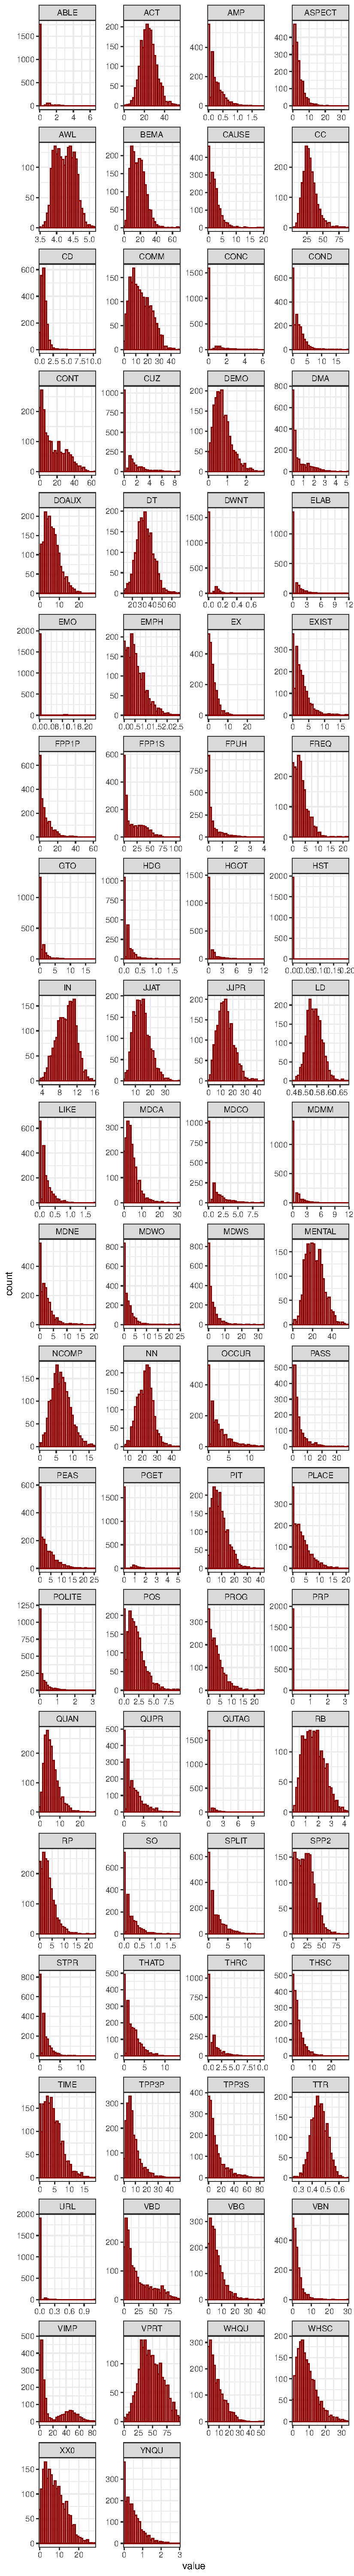
\includegraphics{Ch6_data_prep_files/figure-pdf/distribution-viz-1.pdf}

\begin{Shaded}
\begin{Highlighting}[]
\CommentTok{\#ggsave(here("plots", "TEC{-}HistogramPlotsAllVariablesTEC{-}only.svg"), width = 20, height = 45)}
\end{Highlighting}
\end{Shaded}

\subsection{Feature removal}\label{feature-removal}

A number of features were removed from the dataset as they are not
linguistically interpretable. In the case of the TEC, this included the
variable CD because numbers spellt out as digits were removed from the
textbooks before these were tagged with the MFTE. In addition, the
variables LIKE and SO because these are ``bin'' features included in the
output of the MFTE to ensure that the counts for these polysemous words
do not inflate other categories due to mistags (Le Foll 2021b).

Whenever linguistically meaningful, very low-frequency features were
merged. Finally, features absent from more than third of texts were also
excluded. For the analysis intra-textbook register variation, the
following linguistic features were excluded from the analysis due to low
dispersion:

\begin{Shaded}
\begin{Highlighting}[]
\CommentTok{\# Removal of meaningless features:}
\NormalTok{TxBcounts }\OtherTok{\textless{}{-}}\NormalTok{ TxBcounts }\SpecialCharTok{|\textgreater{}}  
  \FunctionTok{select}\NormalTok{(}\SpecialCharTok{{-}}\FunctionTok{c}\NormalTok{(CD, LIKE, SO))}

\CommentTok{\# Function to compute percentage of texts with occurrences meeting a condition}
\NormalTok{compute\_percentage }\OtherTok{\textless{}{-}} \ControlFlowTok{function}\NormalTok{(data, condition, threshold) \{}
\NormalTok{  numeric\_data }\OtherTok{\textless{}{-}} \FunctionTok{Filter}\NormalTok{(is.numeric, data)}
\NormalTok{  percentage }\OtherTok{\textless{}{-}} \FunctionTok{round}\NormalTok{(}\FunctionTok{colSums}\NormalTok{(condition[, }\FunctionTok{sapply}\NormalTok{(numeric\_data, is.numeric)])}\SpecialCharTok{/}\FunctionTok{nrow}\NormalTok{(data) }\SpecialCharTok{*} \DecValTok{100}\NormalTok{, }\DecValTok{2}\NormalTok{)}
\NormalTok{  percentage }\OtherTok{\textless{}{-}} \FunctionTok{as.data.frame}\NormalTok{(percentage)}
  \FunctionTok{colnames}\NormalTok{(percentage) }\OtherTok{\textless{}{-}} \StringTok{"Percentage"}
\NormalTok{  percentage }\OtherTok{\textless{}{-}}\NormalTok{ percentage }\SpecialCharTok{|\textgreater{}}  
    \FunctionTok{filter}\NormalTok{(}\SpecialCharTok{!}\FunctionTok{is.na}\NormalTok{(Percentage)) }\SpecialCharTok{|\textgreater{}} 
    \FunctionTok{rownames\_to\_column}\NormalTok{() }\SpecialCharTok{|\textgreater{}} 
    \FunctionTok{arrange}\NormalTok{(Percentage)}
  \ControlFlowTok{if}\NormalTok{ (}\SpecialCharTok{!}\FunctionTok{missing}\NormalTok{(threshold)) \{}
\NormalTok{    percentage }\OtherTok{\textless{}{-}}\NormalTok{ percentage }\SpecialCharTok{|\textgreater{}}  
      \FunctionTok{filter}\NormalTok{(Percentage }\SpecialCharTok{\textgreater{}}\NormalTok{ threshold)}
\NormalTok{  \}}
  \FunctionTok{return}\NormalTok{(percentage)}
\NormalTok{\}}

\CommentTok{\# Calculate percentage of texts with 0 occurrences of each feature}
\NormalTok{zero\_features }\OtherTok{\textless{}{-}} \FunctionTok{compute\_percentage}\NormalTok{(TxBcounts, TxBcounts }\SpecialCharTok{==} \DecValTok{0}\NormalTok{, }\FloatTok{66.6}\NormalTok{)}
\CommentTok{\#print(zero\_features)}

\CommentTok{\# Combine low frequency features into meaningful groups whenever this makes linguistic sense}
\NormalTok{TxBcounts }\OtherTok{\textless{}{-}}\NormalTok{ TxBcounts }\SpecialCharTok{|\textgreater{}}  
  \FunctionTok{mutate}\NormalTok{(}\AttributeTok{JJPR =}\NormalTok{ ABLE }\SpecialCharTok{+}\NormalTok{ JJPR, }\AttributeTok{ABLE =} \ConstantTok{NULL}\NormalTok{) }\SpecialCharTok{|\textgreater{}}  
  \FunctionTok{mutate}\NormalTok{(}\AttributeTok{PASS =}\NormalTok{ PGET }\SpecialCharTok{+}\NormalTok{ PASS, }\AttributeTok{PGET =} \ConstantTok{NULL}\NormalTok{)}

\CommentTok{\# Re{-}calculate percentage of texts with 0 occurrences of each feature}
\NormalTok{zero\_features2 }\OtherTok{\textless{}{-}} \FunctionTok{compute\_percentage}\NormalTok{(TxBcounts, TxBcounts }\SpecialCharTok{==} \DecValTok{0}\NormalTok{, }\FloatTok{66.6}\NormalTok{)}
\FunctionTok{print}\NormalTok{(zero\_features2)}
\end{Highlighting}
\end{Shaded}

\begin{verbatim}
   rowname Percentage
1      GTO      67.07
2     ELAB      69.30
3     MDMM      70.81
4     HGOT      73.75
5     CONC      80.48
6     DWNT      81.44
7    QUTAG      85.99
8      URL      96.51
9      EMO      97.82
10     PRP      98.33
11     HST      99.44
\end{verbatim}

\begin{Shaded}
\begin{Highlighting}[]
\CommentTok{\# Drop variables with low document frequency}
\NormalTok{TxBcounts }\OtherTok{\textless{}{-}} \FunctionTok{select}\NormalTok{(TxBcounts, }\SpecialCharTok{{-}}\FunctionTok{one\_of}\NormalTok{(zero\_features2}\SpecialCharTok{$}\NormalTok{rowname))}
\CommentTok{\#ncol(TxBcounts){-}8 \# Number of linguistic features remaining}

\CommentTok{\# List of features}
\CommentTok{\#colnames(TxBcounts)}
\end{Highlighting}
\end{Shaded}

These feature removal operations resulted in a feature set of 64
linguistic variables.

\subsection{Identifying potential outlier
texts}\label{identifying-potential-outlier-texts}

All normalised frequencies were normalised to identify any potential
outlier texts.

\begin{Shaded}
\begin{Highlighting}[]
\CommentTok{\# First scale the normalised counts (z{-}standardisation) to be able to compare the various features}
\NormalTok{TxBcounts }\SpecialCharTok{|\textgreater{}} 
  \FunctionTok{select}\NormalTok{(}\SpecialCharTok{{-}}\NormalTok{Words) }\SpecialCharTok{|\textgreater{}}  
  \FunctionTok{keep}\NormalTok{(is.numeric) }\SpecialCharTok{|\textgreater{}}  
  \FunctionTok{scale}\NormalTok{() }\OtherTok{{-}\textgreater{}}
\NormalTok{  TxBzcounts}

\FunctionTok{boxplot}\NormalTok{(TxBzcounts, }\AttributeTok{las =} \DecValTok{3}\NormalTok{, }\AttributeTok{main =} \StringTok{"z{-}scores"}\NormalTok{) }\CommentTok{\# Slow to open!}
\end{Highlighting}
\end{Shaded}

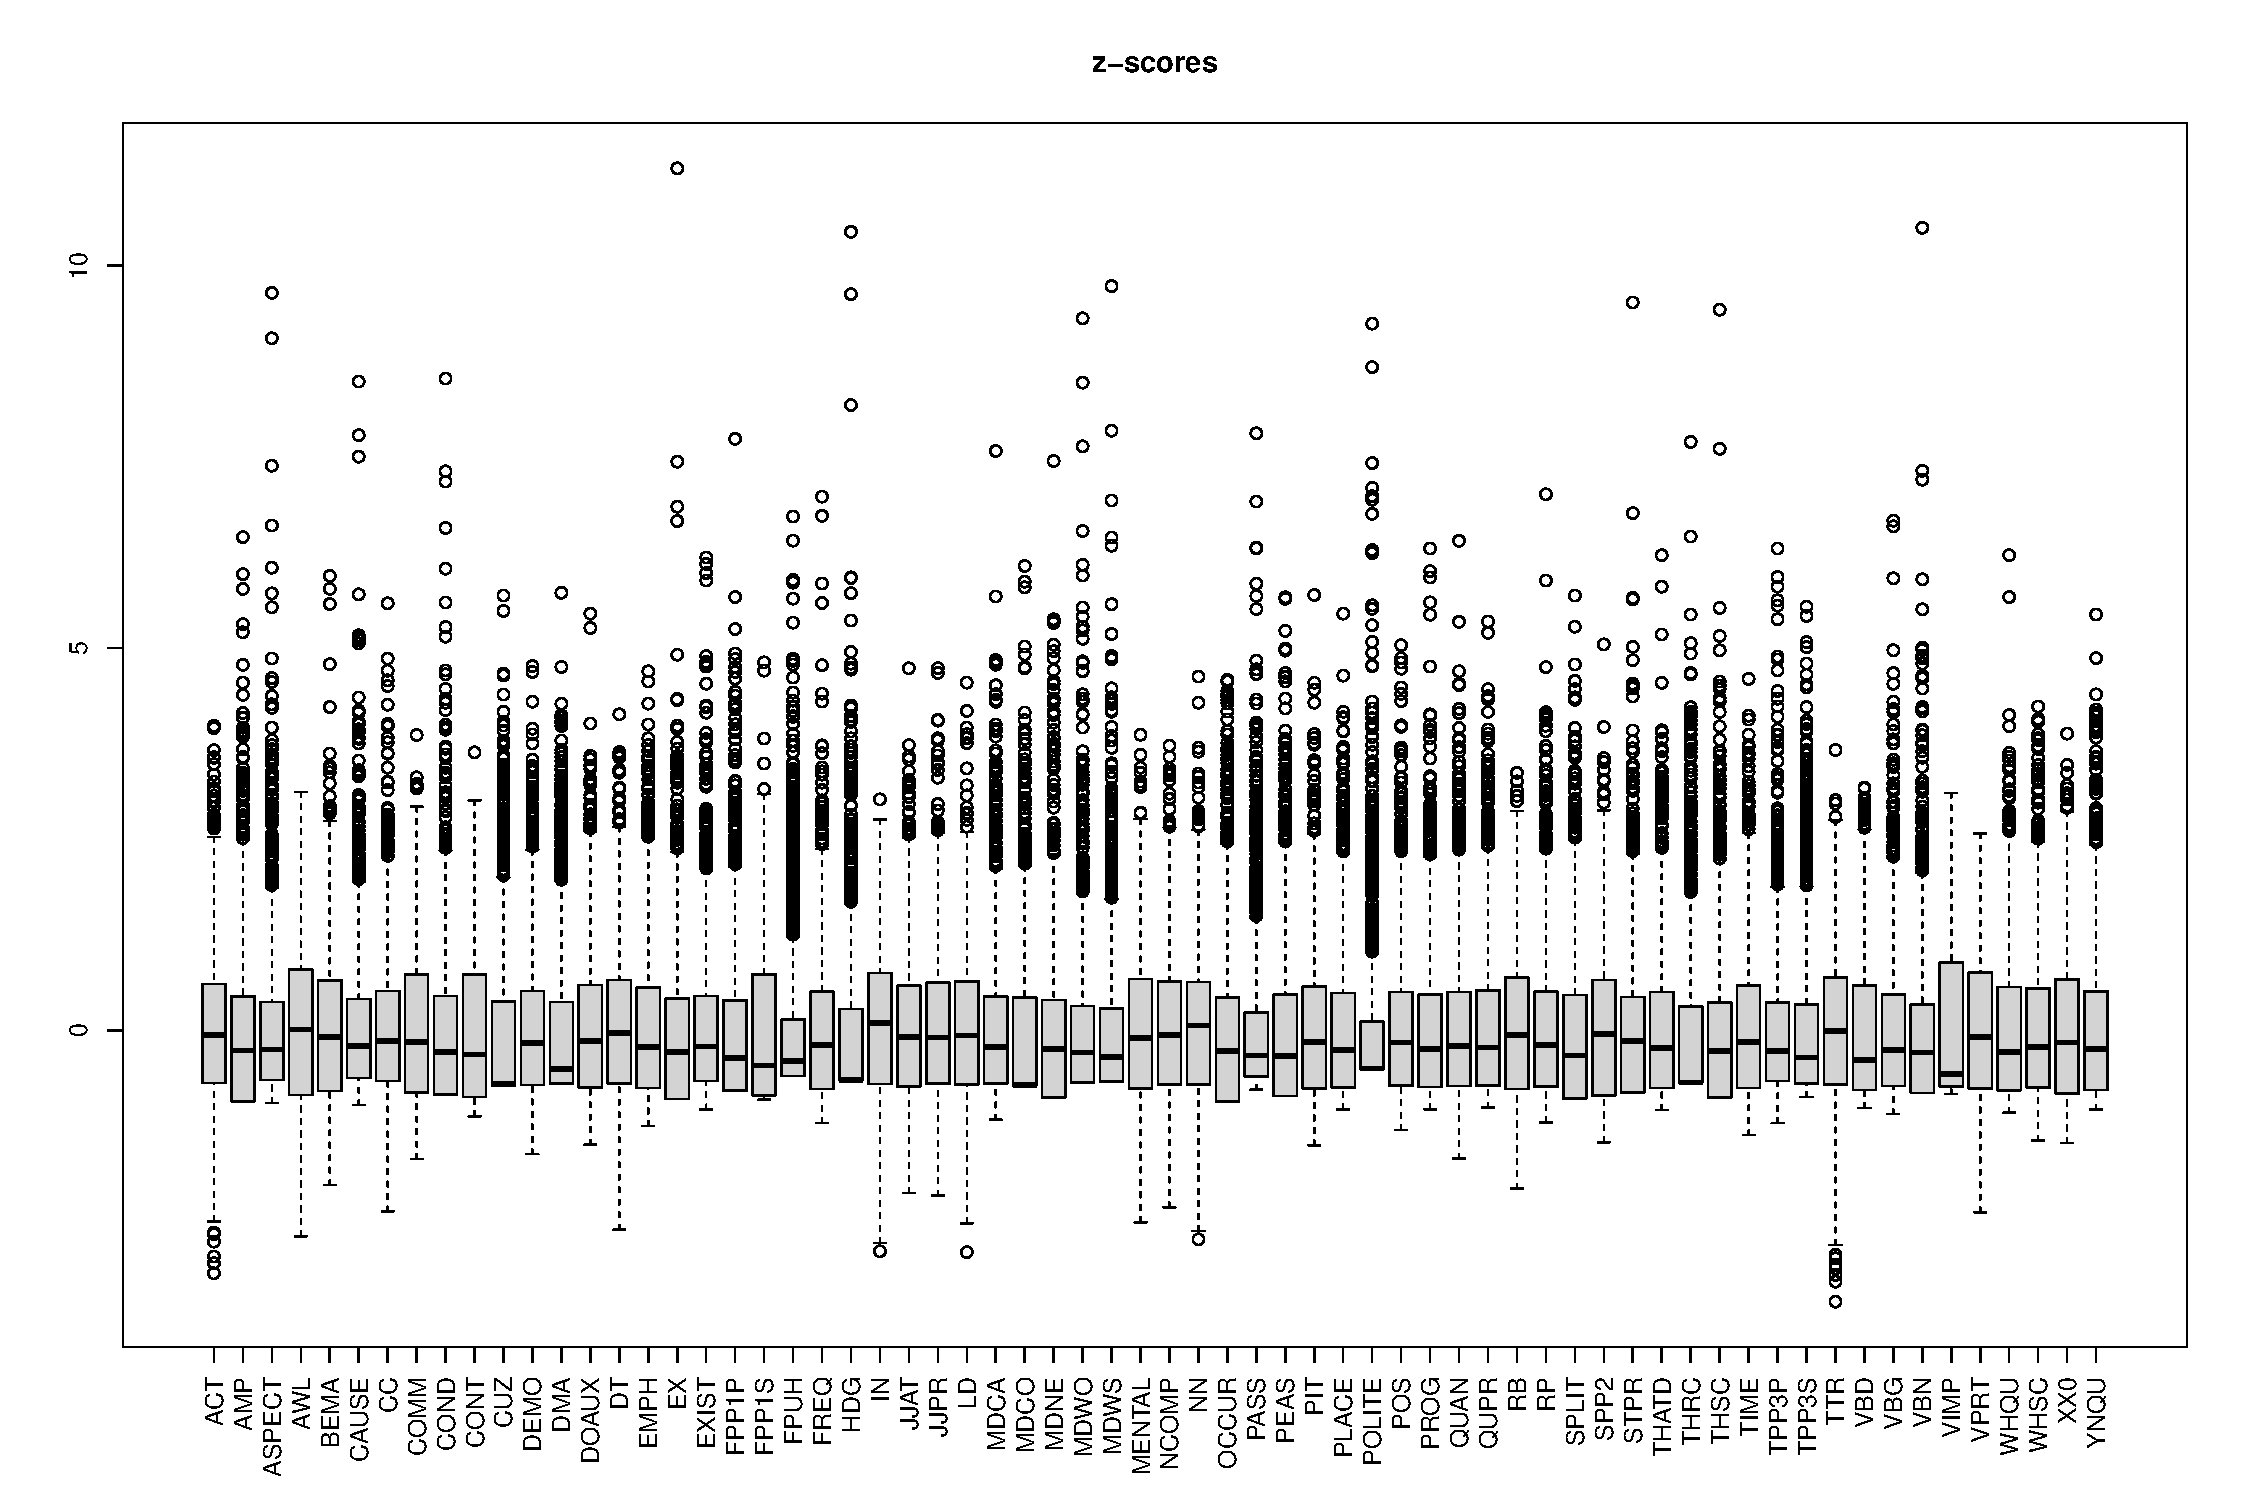
\includegraphics{Ch6_data_prep_files/figure-pdf/z-standardisation-outliers-1.pdf}

\begin{Shaded}
\begin{Highlighting}[]
\CommentTok{\# If necessary, remove any outliers at this stage.}
\NormalTok{TxBdata }\OtherTok{\textless{}{-}} \FunctionTok{cbind}\NormalTok{(TxBcounts[,}\DecValTok{1}\SpecialCharTok{:}\DecValTok{6}\NormalTok{], }\FunctionTok{as.data.frame}\NormalTok{(TxBzcounts))}

\NormalTok{outliers }\OtherTok{\textless{}{-}}\NormalTok{ TxBdata }\SpecialCharTok{|\textgreater{}}  
  \FunctionTok{select}\NormalTok{(}\SpecialCharTok{{-}}\FunctionTok{c}\NormalTok{(Words, LD, TTR)) }\SpecialCharTok{|\textgreater{}}  
  \FunctionTok{filter}\NormalTok{(}\FunctionTok{if\_any}\NormalTok{(}\FunctionTok{where}\NormalTok{(is.numeric), }\SpecialCharTok{\textasciitilde{}}\NormalTok{ .x }\SpecialCharTok{\textgreater{}} \DecValTok{8}\NormalTok{)) }\SpecialCharTok{|\textgreater{}}  
  \FunctionTok{select}\NormalTok{(Filename)}
\end{Highlighting}
\end{Shaded}

The following outlier texts were identified and excluded in subsequent
analyses.

\begin{Shaded}
\begin{Highlighting}[]
\NormalTok{outliers}
\end{Highlighting}
\end{Shaded}

\begin{verbatim}
                                            Filename
1                             POC_4e_Spoken_0007.txt
2             Solutions_Elementary_Personal_0001.txt
3                       NGL_5_Instructional_0018.txt
4                           Access_1_Spoken_0011.txt
5                              EIM_1_Spoken_0012.txt
6                              NGL_4_Spoken_0011.txt
7      Solutions_Intermediate_Plus_Personal_0001.txt
8           Solutions_Elementary_ELF_Spoken_0021.txt
9                          NB_2_Informative_0009.txt
10       Solutions_Intermediate_Plus_Spoken_0022.txt
11     Solutions_Intermediate_Instructional_0025.txt
12 Solutions_Pre-Intermediate_Instructional_0024.txt
13                            POC_4e_Spoken_0010.txt
14            Solutions_Intermediate_Spoken_0019.txt
15                          Access_1_Spoken_0019.txt
16    Solutions_Pre-Intermediate_ELF_Spoken_0005.txt
\end{verbatim}

\begin{Shaded}
\begin{Highlighting}[]
\NormalTok{TxBcounts }\OtherTok{\textless{}{-}}\NormalTok{ TxBcounts }\SpecialCharTok{|\textgreater{}}  
  \FunctionTok{filter}\NormalTok{(}\SpecialCharTok{!}\NormalTok{Filename }\SpecialCharTok{\%in\%}\NormalTok{ outliers}\SpecialCharTok{$}\NormalTok{Filename)}

\NormalTok{TxBcounts }\SpecialCharTok{|\textgreater{}} 
  \FunctionTok{select}\NormalTok{(}\SpecialCharTok{{-}}\NormalTok{Words) }\SpecialCharTok{|\textgreater{}}  
  \FunctionTok{keep}\NormalTok{(is.numeric) }\SpecialCharTok{|\textgreater{}}  
  \FunctionTok{scale}\NormalTok{() }\OtherTok{{-}\textgreater{}}
\NormalTok{  TxBzcounts}
\end{Highlighting}
\end{Shaded}

This resulted in 1,961 TEC texts being included in the model of
intra-textbook linguistic variation with the following normalised
feature distributions.

\begin{Shaded}
\begin{Highlighting}[]
\NormalTok{TxBzcounts }\SpecialCharTok{|\textgreater{}} 
  \FunctionTok{as.data.frame}\NormalTok{() }\SpecialCharTok{|\textgreater{}}  
  \FunctionTok{gather}\NormalTok{() }\SpecialCharTok{|\textgreater{}}  \CommentTok{\# This function from tidyr converts a selection of variables into two variables: a key and a value. The key contains the names of the original variable and the value the data. This means we can then use the facet\_wrap function from ggplot2}
  \FunctionTok{ggplot}\NormalTok{(}\FunctionTok{aes}\NormalTok{(value)) }\SpecialCharTok{+}
    \FunctionTok{theme\_bw}\NormalTok{() }\SpecialCharTok{+}
    \FunctionTok{facet\_wrap}\NormalTok{(}\SpecialCharTok{\textasciitilde{}}\NormalTok{ key, }\AttributeTok{scales =} \StringTok{"free"}\NormalTok{, }\AttributeTok{ncol =} \DecValTok{4}\NormalTok{) }\SpecialCharTok{+}
    \FunctionTok{scale\_x\_continuous}\NormalTok{(}\AttributeTok{expand=}\FunctionTok{c}\NormalTok{(}\DecValTok{0}\NormalTok{,}\DecValTok{0}\NormalTok{)) }\SpecialCharTok{+}
    \FunctionTok{geom\_histogram}\NormalTok{(}\AttributeTok{bins =} \DecValTok{30}\NormalTok{, }\AttributeTok{colour=} \StringTok{"darkred"}\NormalTok{, }\AttributeTok{fill =} \StringTok{"darkred"}\NormalTok{, }\AttributeTok{alpha =} \FloatTok{0.5}\NormalTok{)}
\end{Highlighting}
\end{Shaded}

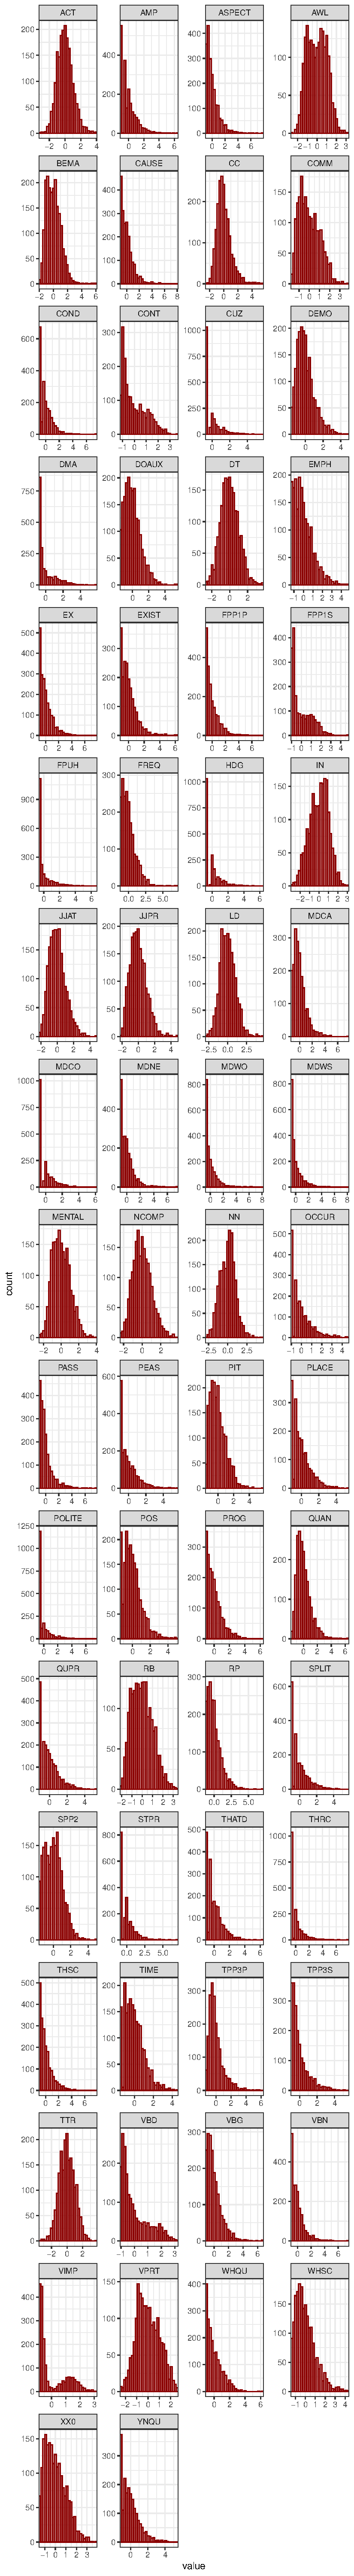
\includegraphics{Ch6_data_prep_files/figure-pdf/z-transformed-distributions-1.pdf}

\begin{Shaded}
\begin{Highlighting}[]
\CommentTok{\#ggsave(here("plots", "TEC{-}zscores{-}HistogramsAllVariablesTEC{-}only.svg"), width = 20, height = 45)}
\end{Highlighting}
\end{Shaded}

\subsection{Signed log transformation}\label{signed-log-transformation}

A signed logarithmic transformation was applied to (further) deskew the
feature distributions (Diwersy, Evert, and Neumann 2014; Neumann and
Evert 2021).

The signed log transformation function was inspired by the SignedLog
function proposed in
https://cran.r-project.org/web/packages/DataVisualizations/DataVisualizations.pdf

\begin{Shaded}
\begin{Highlighting}[]
\CommentTok{\# All features are signed log{-}transformed (note that this is also what Neumann \& Evert 2021 propose)}
\NormalTok{signed.log }\OtherTok{\textless{}{-}} \ControlFlowTok{function}\NormalTok{(x) \{}
  \FunctionTok{sign}\NormalTok{(x) }\SpecialCharTok{*} \FunctionTok{log}\NormalTok{(}\FunctionTok{abs}\NormalTok{(x) }\SpecialCharTok{+} \DecValTok{1}\NormalTok{)}
\NormalTok{  \}}

\NormalTok{TxBzlogcounts }\OtherTok{\textless{}{-}} \FunctionTok{signed.log}\NormalTok{(TxBzcounts) }\CommentTok{\# Standardise first, then signed log transform}

\CommentTok{\#saveRDS(TxBzlogcounts, here("processed\_data", "TxBzlogcounts.rds")) \# Last saved 16 Feb 2024}
\end{Highlighting}
\end{Shaded}

The new feature distributions are visualised below.

\begin{Shaded}
\begin{Highlighting}[]
\NormalTok{TxBzlogcounts }\SpecialCharTok{|\textgreater{}} 
  \FunctionTok{as.data.frame}\NormalTok{() }\SpecialCharTok{|\textgreater{}}  
  \FunctionTok{gather}\NormalTok{() }\SpecialCharTok{|\textgreater{}}  \CommentTok{\# This function from tidyr converts a selection of variables into two variables: a key and a value. The key contains the names of the original variable and the value the data. This means we can then use the facet\_wrap function from ggplot2}
  \FunctionTok{ggplot}\NormalTok{(}\FunctionTok{aes}\NormalTok{(value, }\FunctionTok{after\_stat}\NormalTok{(density))) }\SpecialCharTok{+}
  \FunctionTok{theme\_bw}\NormalTok{() }\SpecialCharTok{+}
  \FunctionTok{facet\_wrap}\NormalTok{(}\SpecialCharTok{\textasciitilde{}}\NormalTok{ key, }\AttributeTok{scales =} \StringTok{"free"}\NormalTok{, }\AttributeTok{ncol =} \DecValTok{4}\NormalTok{) }\SpecialCharTok{+}
  \FunctionTok{scale\_x\_continuous}\NormalTok{(}\AttributeTok{expand=}\FunctionTok{c}\NormalTok{(}\DecValTok{0}\NormalTok{,}\DecValTok{0}\NormalTok{)) }\SpecialCharTok{+}
  \FunctionTok{scale\_y\_continuous}\NormalTok{(}\AttributeTok{limits =} \FunctionTok{c}\NormalTok{(}\DecValTok{0}\NormalTok{,}\ConstantTok{NA}\NormalTok{)) }\SpecialCharTok{+}
  \FunctionTok{geom\_histogram}\NormalTok{(}\AttributeTok{bins =} \DecValTok{30}\NormalTok{, }\AttributeTok{colour=} \StringTok{"black"}\NormalTok{, }\AttributeTok{fill =} \StringTok{"grey"}\NormalTok{) }\SpecialCharTok{+}
  \FunctionTok{geom\_density}\NormalTok{(}\AttributeTok{colour =} \StringTok{"darkred"}\NormalTok{, }\AttributeTok{weight =} \DecValTok{2}\NormalTok{, }\AttributeTok{fill=}\StringTok{"darkred"}\NormalTok{, }\AttributeTok{alpha =}\NormalTok{ .}\DecValTok{4}\NormalTok{)}
\end{Highlighting}
\end{Shaded}

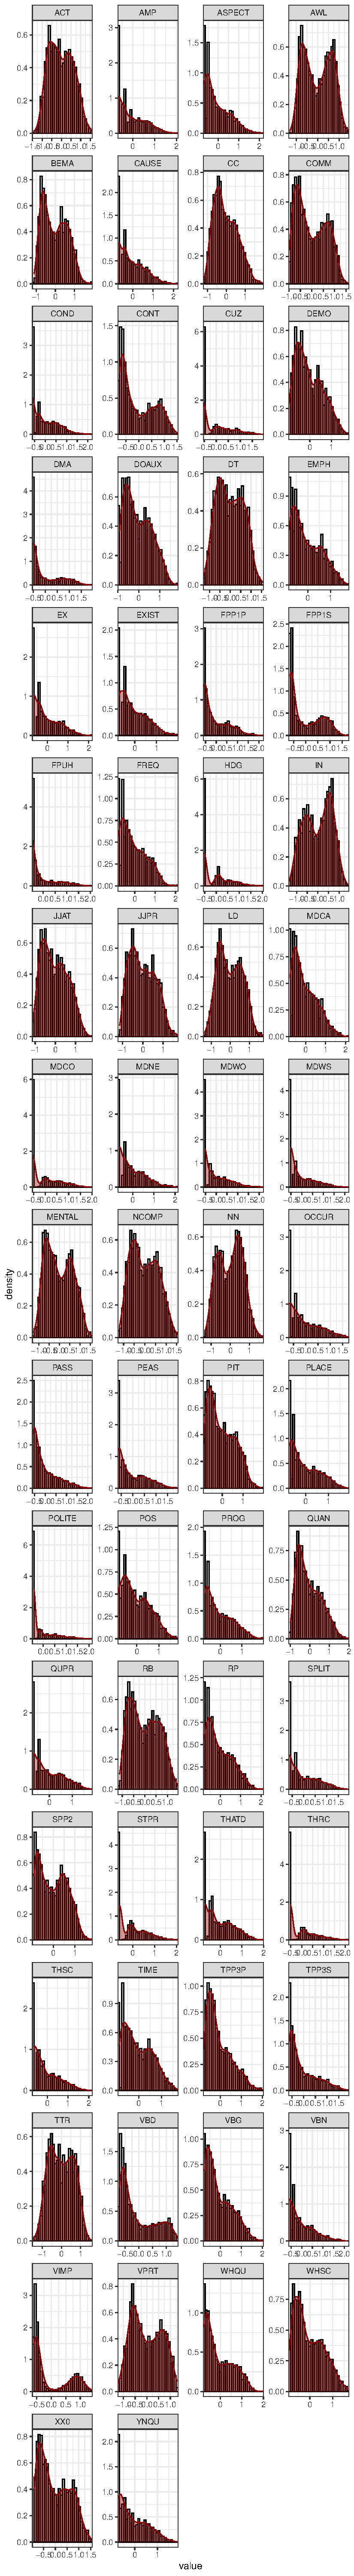
\includegraphics{Ch6_data_prep_files/figure-pdf/signed.log.transformation-distributions-1.pdf}

\begin{Shaded}
\begin{Highlighting}[]
\CommentTok{\#ggsave(here("plots", "DensityPlotsAllVariablesSignedLog{-}TEC{-}only.svg"), width = 15, height = 49)}
\end{Highlighting}
\end{Shaded}

The following correlation plots serve to illustrate the effect of the
variable transformations performed in the above chunks.

Example feature distributions before transformations:

\begin{Shaded}
\begin{Highlighting}[]
\CommentTok{\# This is a slightly amended version of the PerformanceAnalytics::chart.Correlation() function. It simply removes the significance stars that are meaningless with this many data points (see commented out lines below)}

\NormalTok{chart.Correlation.nostars }\OtherTok{\textless{}{-}} \ControlFlowTok{function}\NormalTok{ (R, }\AttributeTok{histogram =} \ConstantTok{TRUE}\NormalTok{, }\AttributeTok{method =} \FunctionTok{c}\NormalTok{(}\StringTok{"pearson"}\NormalTok{, }\StringTok{"kendall"}\NormalTok{, }\StringTok{"spearman"}\NormalTok{), ...) \{}
\NormalTok{  x }\OtherTok{=} \FunctionTok{checkData}\NormalTok{(R, }\AttributeTok{method =} \StringTok{"matrix"}\NormalTok{)}
  \ControlFlowTok{if}\NormalTok{ (}\FunctionTok{missing}\NormalTok{(method)) }
\NormalTok{    method }\OtherTok{=}\NormalTok{ method[}\DecValTok{1}\NormalTok{]}
\NormalTok{  panel.cor }\OtherTok{\textless{}{-}} \ControlFlowTok{function}\NormalTok{(x, y, }\AttributeTok{digits =} \DecValTok{2}\NormalTok{, }\AttributeTok{prefix =} \StringTok{""}\NormalTok{, }\AttributeTok{use =} \StringTok{"pairwise.complete.obs"}\NormalTok{, }\AttributeTok{method =} \StringTok{"pearson"}\NormalTok{, cex.cor, ...) \{}
\NormalTok{    usr }\OtherTok{\textless{}{-}} \FunctionTok{par}\NormalTok{(}\StringTok{"usr"}\NormalTok{)}
    \FunctionTok{on.exit}\NormalTok{(}\FunctionTok{par}\NormalTok{(usr))}
    \FunctionTok{par}\NormalTok{(}\AttributeTok{usr =} \FunctionTok{c}\NormalTok{(}\DecValTok{0}\NormalTok{, }\DecValTok{1}\NormalTok{, }\DecValTok{0}\NormalTok{, }\DecValTok{1}\NormalTok{))}
\NormalTok{    r }\OtherTok{\textless{}{-}} \FunctionTok{cor}\NormalTok{(x, y, }\AttributeTok{use =}\NormalTok{ use, }\AttributeTok{method =}\NormalTok{ method)}
\NormalTok{    txt }\OtherTok{\textless{}{-}} \FunctionTok{format}\NormalTok{(}\FunctionTok{c}\NormalTok{(r, }\FloatTok{0.123456789}\NormalTok{), }\AttributeTok{digits =}\NormalTok{ digits)[}\DecValTok{1}\NormalTok{]}
\NormalTok{    txt }\OtherTok{\textless{}{-}} \FunctionTok{paste}\NormalTok{(prefix, txt, }\AttributeTok{sep =} \StringTok{""}\NormalTok{)}
    \ControlFlowTok{if}\NormalTok{ (}\FunctionTok{missing}\NormalTok{(cex.cor)) }
\NormalTok{      cex }\OtherTok{\textless{}{-}} \FloatTok{0.8}\SpecialCharTok{/}\FunctionTok{strwidth}\NormalTok{(txt)}
\NormalTok{    test }\OtherTok{\textless{}{-}} \FunctionTok{cor.test}\NormalTok{(}\FunctionTok{as.numeric}\NormalTok{(x), }\FunctionTok{as.numeric}\NormalTok{(y), }\AttributeTok{method =}\NormalTok{ method)}
    \CommentTok{\# Signif \textless{}{-} symnum(test$p.value, corr = FALSE, na = FALSE, }
    \CommentTok{\#                  cutpoints = c(0, 0.001, 0.01, 0.05, 0.1, 1), symbols = c("***", }
    \CommentTok{\#                                                                           "**", "*", ".", " "))}
    \FunctionTok{text}\NormalTok{(}\FloatTok{0.5}\NormalTok{, }\FloatTok{0.5}\NormalTok{, txt, }\AttributeTok{cex =}\NormalTok{ cex }\SpecialCharTok{*}\NormalTok{ (}\FunctionTok{abs}\NormalTok{(r) }\SpecialCharTok{+} \FloatTok{0.3}\NormalTok{)}\SpecialCharTok{/}\FloatTok{1.3}\NormalTok{)}
    \CommentTok{\# text(0.8, 0.8, Signif, cex = cex, col = 2)}
\NormalTok{  \}}
\NormalTok{  f }\OtherTok{\textless{}{-}} \ControlFlowTok{function}\NormalTok{(t) \{}
    \FunctionTok{dnorm}\NormalTok{(t, }\AttributeTok{mean =} \FunctionTok{mean}\NormalTok{(x), }\AttributeTok{sd =} \FunctionTok{sd.xts}\NormalTok{(x))}
\NormalTok{  \}}
\NormalTok{  dotargs }\OtherTok{\textless{}{-}} \FunctionTok{list}\NormalTok{(...)}
\NormalTok{  dotargs}\SpecialCharTok{$}\NormalTok{method }\OtherTok{\textless{}{-}} \ConstantTok{NULL}
  \FunctionTok{rm}\NormalTok{(method)}
\NormalTok{  hist.panel }\OtherTok{=} \ControlFlowTok{function}\NormalTok{(x, }\AttributeTok{... =} \ConstantTok{NULL}\NormalTok{) \{}
    \FunctionTok{par}\NormalTok{(}\AttributeTok{new =} \ConstantTok{TRUE}\NormalTok{)}
    \FunctionTok{hist}\NormalTok{(x, }\AttributeTok{col =} \StringTok{"light gray"}\NormalTok{, }\AttributeTok{probability =} \ConstantTok{TRUE}\NormalTok{, }
         \AttributeTok{axes =} \ConstantTok{FALSE}\NormalTok{, }\AttributeTok{main =} \StringTok{""}\NormalTok{, }\AttributeTok{breaks =} \StringTok{"FD"}\NormalTok{)}
    \FunctionTok{lines}\NormalTok{(}\FunctionTok{density}\NormalTok{(x, }\AttributeTok{na.rm =} \ConstantTok{TRUE}\NormalTok{), }\AttributeTok{col =} \StringTok{"red"}\NormalTok{, }\AttributeTok{lwd =} \DecValTok{1}\NormalTok{)}
    \FunctionTok{rug}\NormalTok{(x)}
\NormalTok{  \}}
  \ControlFlowTok{if}\NormalTok{ (histogram) }
    \FunctionTok{pairs}\NormalTok{(x, }\AttributeTok{gap =} \DecValTok{0}\NormalTok{, }\AttributeTok{lower.panel =}\NormalTok{ panel.smooth, }\AttributeTok{upper.panel =}\NormalTok{ panel.cor, }
          \AttributeTok{diag.panel =}\NormalTok{ hist.panel)}
  \ControlFlowTok{else} \FunctionTok{pairs}\NormalTok{(x, }\AttributeTok{gap =} \DecValTok{0}\NormalTok{, }\AttributeTok{lower.panel =}\NormalTok{ panel.smooth, }\AttributeTok{upper.panel =}\NormalTok{ panel.cor)}
\NormalTok{\}}

\CommentTok{\# Example plot without any variable transformation}
\NormalTok{example1 }\OtherTok{\textless{}{-}}\NormalTok{ TxBcounts }\SpecialCharTok{|\textgreater{}} 
  \FunctionTok{select}\NormalTok{(NN,PROG,SPLIT,ACT,FPP1S)}

\CommentTok{\#png(here("plots", "CorrChart{-}TEC{-}examples{-}normedcounts.png"), width = 20, height = 20, units = "cm", res = 300)}
\FunctionTok{chart.Correlation.nostars}\NormalTok{(example1, }\AttributeTok{histogram=}\ConstantTok{TRUE}\NormalTok{, }\AttributeTok{pch=}\DecValTok{19}\NormalTok{)}
\end{Highlighting}
\end{Shaded}

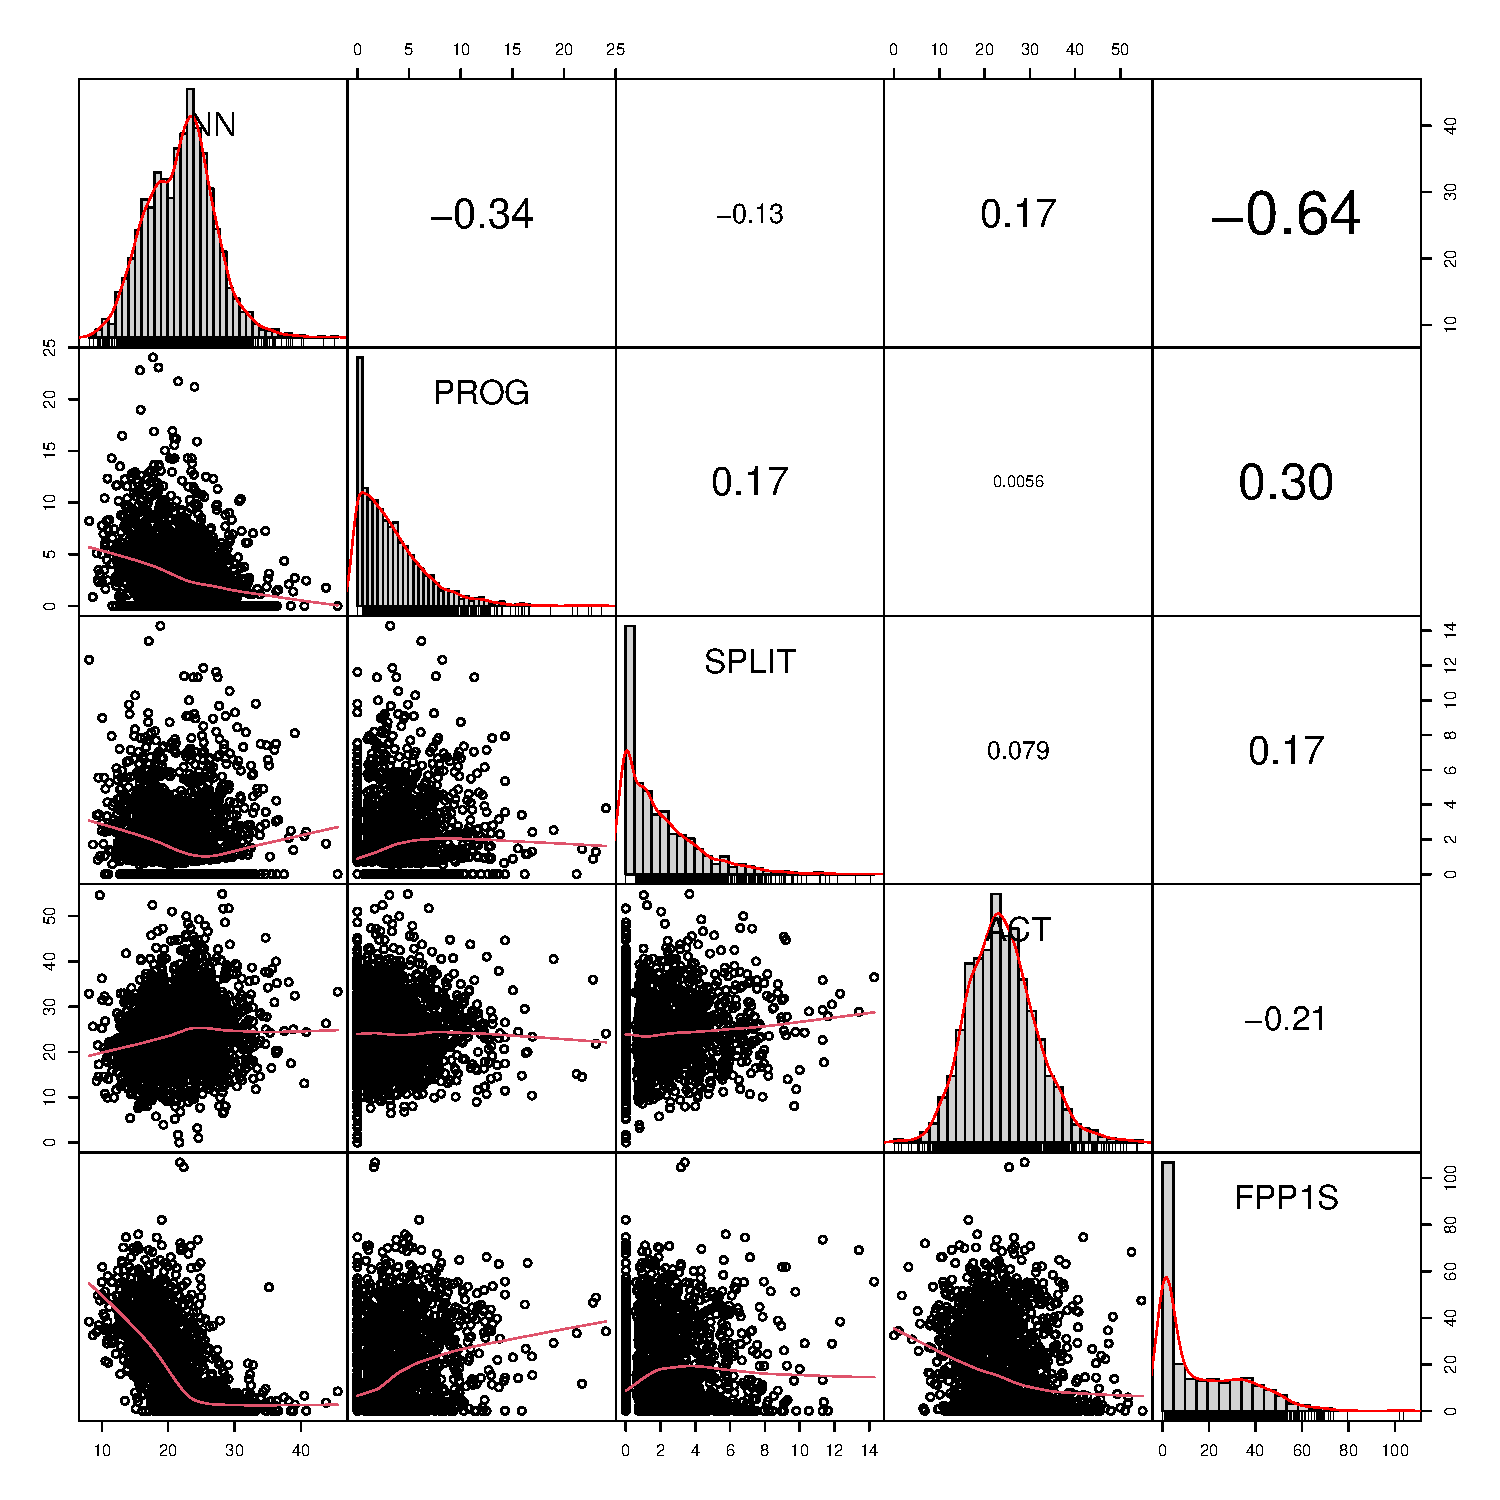
\includegraphics{Ch6_data_prep_files/figure-pdf/example-correlation-plots-1.pdf}

\begin{Shaded}
\begin{Highlighting}[]
\CommentTok{\#dev.off()}
\end{Highlighting}
\end{Shaded}

Example feature distributions after transformations:

\begin{Shaded}
\begin{Highlighting}[]
\CommentTok{\# Example plot with transformed variables}
\NormalTok{example2 }\OtherTok{\textless{}{-}}\NormalTok{ TxBzlogcounts }\SpecialCharTok{|\textgreater{}} 
  \FunctionTok{as.data.frame}\NormalTok{() }\SpecialCharTok{|\textgreater{}}  
  \FunctionTok{select}\NormalTok{(NN,PROG,SPLIT,ACT,FPP1S)}

\CommentTok{\#png(here("plots", "CorrChart{-}TEC{-}examples{-}zsignedlogcounts.png"), width = 20, height = 20, units = "cm", res = 300)}
\FunctionTok{chart.Correlation.nostars}\NormalTok{(example2, }\AttributeTok{histogram=}\ConstantTok{TRUE}\NormalTok{, }\AttributeTok{pch=}\DecValTok{19}\NormalTok{)}
\end{Highlighting}
\end{Shaded}

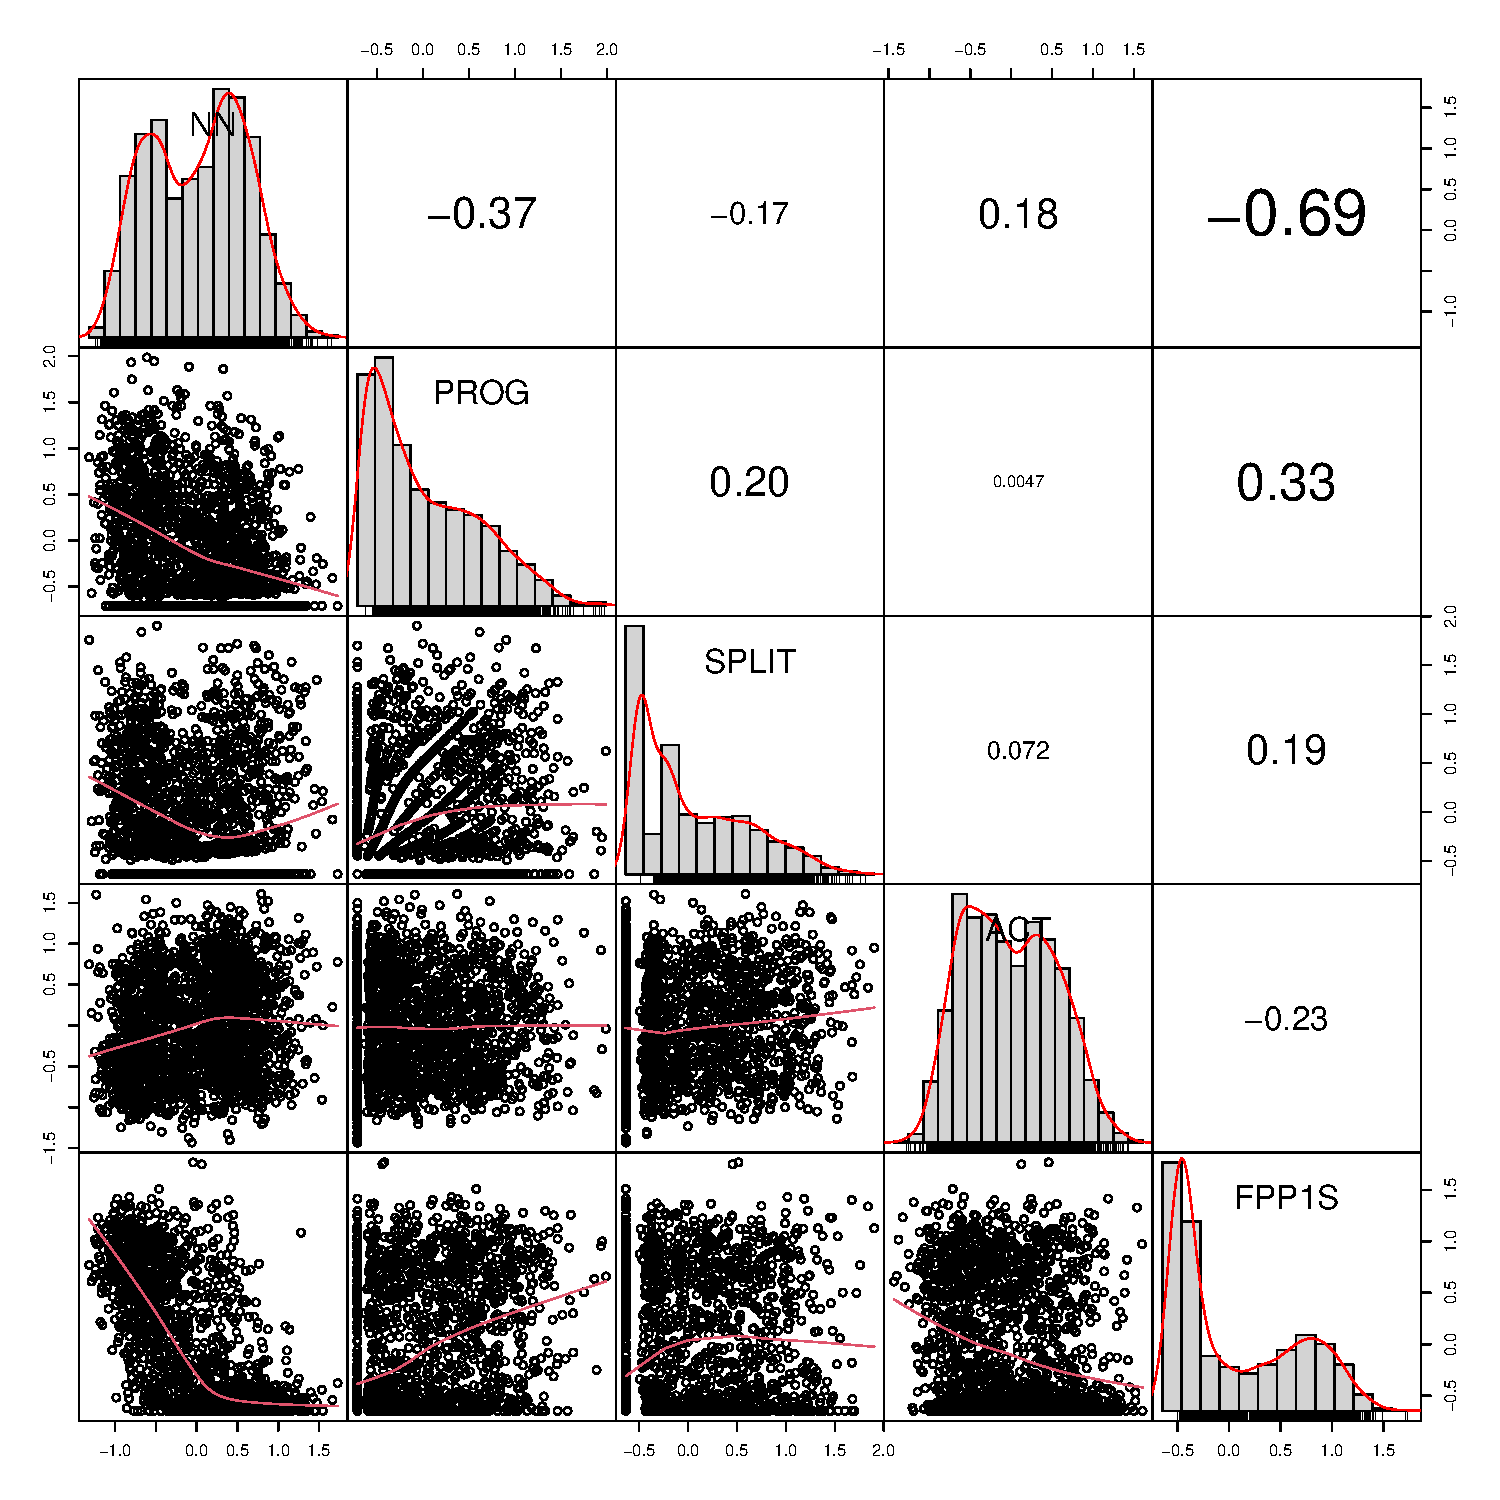
\includegraphics{Ch6_data_prep_files/figure-pdf/example-correlation-plots2-1.pdf}

\begin{Shaded}
\begin{Highlighting}[]
\CommentTok{\#dev.off()}
\end{Highlighting}
\end{Shaded}

\subsection{Feature correlations}\label{feature-correlations}

The correlations of the transformed feature frequencies can be
visualised in the form of a heatmap. Negative correlations are rendered
in blue, whereas positive ones are in red.

\begin{Shaded}
\begin{Highlighting}[]
\CommentTok{\# Simple heatmap in base R (inspired by Stephanie Evert\textquotesingle{}s SIGIL code)}
\NormalTok{cor.colours }\OtherTok{\textless{}{-}} \FunctionTok{c}\NormalTok{(}
  \FunctionTok{hsv}\NormalTok{(}\AttributeTok{h=}\DecValTok{2}\SpecialCharTok{/}\DecValTok{3}\NormalTok{, }\AttributeTok{v=}\DecValTok{1}\NormalTok{, }\AttributeTok{s=}\NormalTok{(}\DecValTok{10}\SpecialCharTok{:}\DecValTok{1}\NormalTok{)}\SpecialCharTok{/}\DecValTok{10}\NormalTok{), }\CommentTok{\# blue = negative correlation }
  \FunctionTok{rgb}\NormalTok{(}\DecValTok{1}\NormalTok{,}\DecValTok{1}\NormalTok{,}\DecValTok{1}\NormalTok{), }\CommentTok{\# white = no correlation }
  \FunctionTok{hsv}\NormalTok{(}\AttributeTok{h=}\DecValTok{0}\NormalTok{, }\AttributeTok{v=}\DecValTok{1}\NormalTok{, }\AttributeTok{s=}\NormalTok{(}\DecValTok{1}\SpecialCharTok{:}\DecValTok{10}\SpecialCharTok{/}\DecValTok{10}\NormalTok{))) }\CommentTok{\# red = positive correlation}

\CommentTok{\#png(here("plots", "heatmapzlogcounts{-}TEC{-}only.png"), width = 30, height= 30, units = "cm", res = 300)}
\FunctionTok{heatmap}\NormalTok{(}\FunctionTok{cor}\NormalTok{(TxBzlogcounts), }
        \AttributeTok{symm=}\ConstantTok{TRUE}\NormalTok{, }
        \AttributeTok{zlim=}\FunctionTok{c}\NormalTok{(}\SpecialCharTok{{-}}\DecValTok{1}\NormalTok{,}\DecValTok{1}\NormalTok{), }
        \AttributeTok{col=}\NormalTok{cor.colours, }
        \AttributeTok{margins=}\FunctionTok{c}\NormalTok{(}\DecValTok{0}\NormalTok{,}\DecValTok{0}\NormalTok{))}
\end{Highlighting}
\end{Shaded}

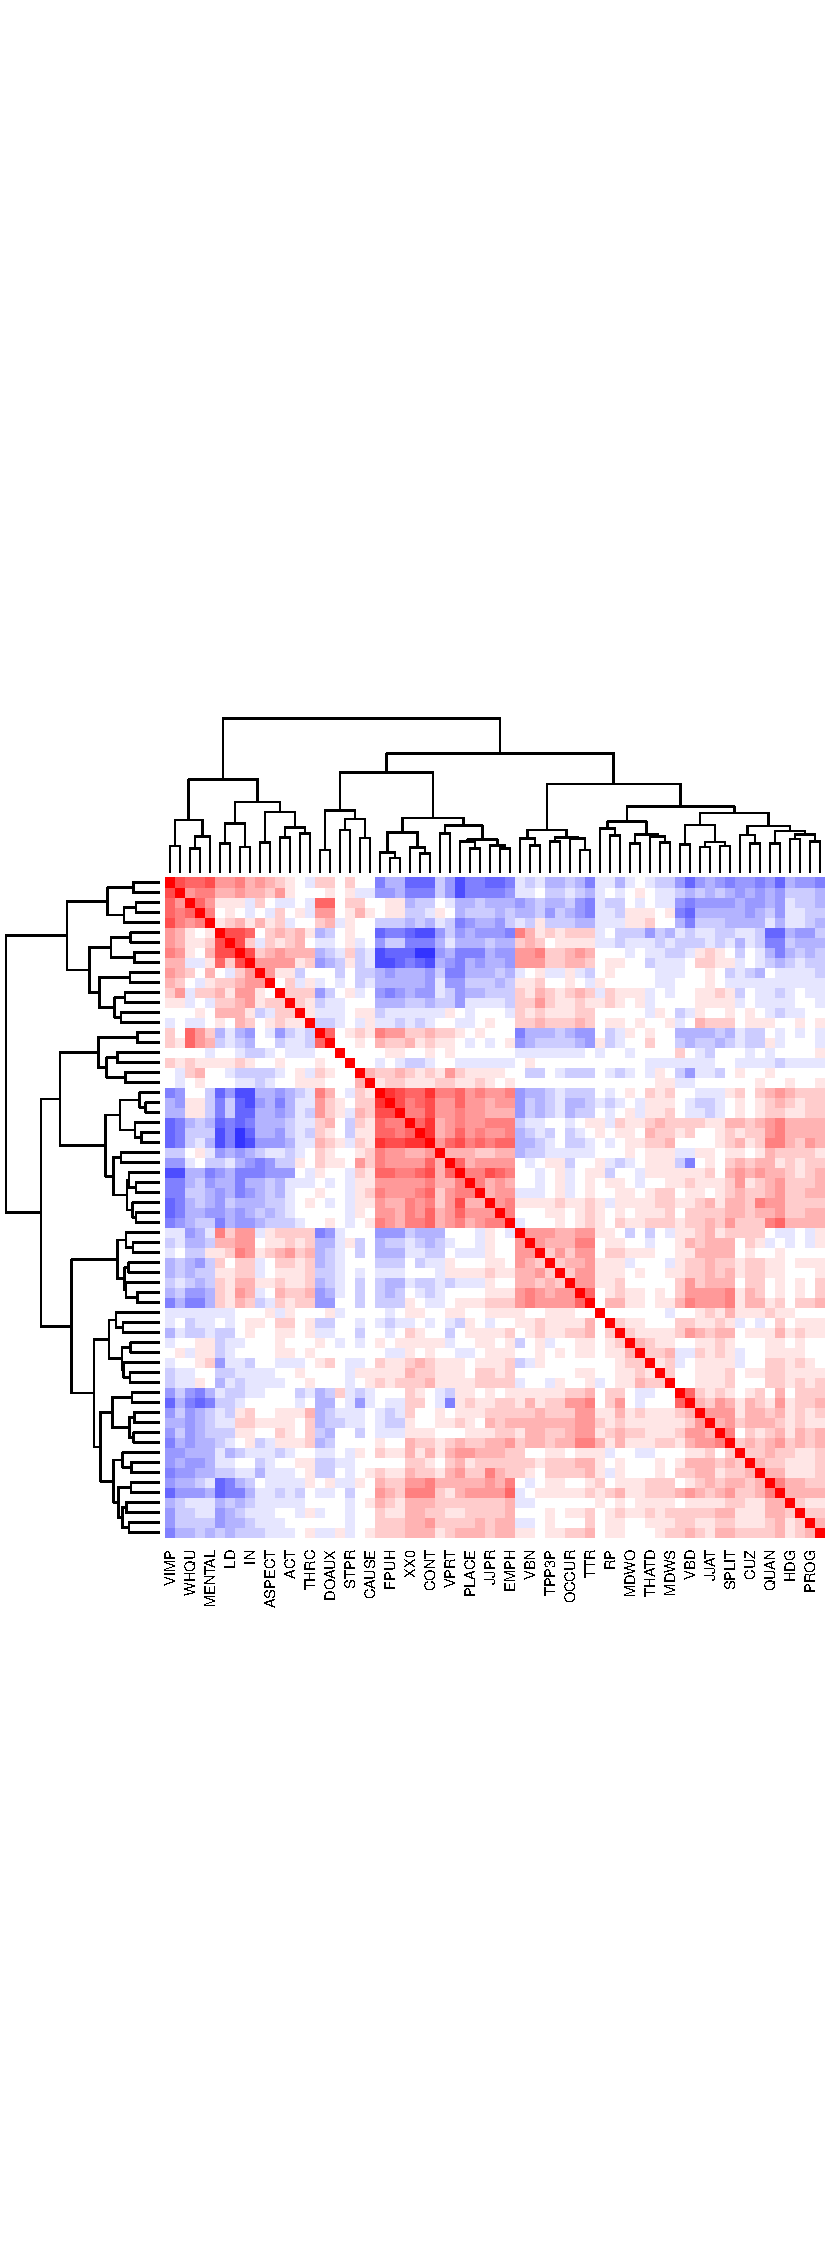
\includegraphics{Ch6_data_prep_files/figure-pdf/heatmap-1.pdf}

\begin{Shaded}
\begin{Highlighting}[]
\CommentTok{\#dev.off()}

\CommentTok{\# Calculate the sum of all the words in the tagged texts of the TEC}
\NormalTok{totalwords }\OtherTok{\textless{}{-}}\NormalTok{ TxBcounts }\SpecialCharTok{|\textgreater{}}  
  \FunctionTok{select}\NormalTok{(Words) }\SpecialCharTok{|\textgreater{}} 
  \FunctionTok{sum}\NormalTok{() }\SpecialCharTok{|\textgreater{}} 
  \FunctionTok{format}\NormalTok{(}\AttributeTok{big.mark=}\StringTok{","}\NormalTok{)}
\end{Highlighting}
\end{Shaded}

\section{Composition of TEC
texts/files}\label{composition-of-tec-textsfiles}

These figures and tables provide summary statistics on the texts/files
of the TEC that were entered in the multi-dimensional model of
intra-textbook linguistic variation. In total, the TEC texts entered
amounted to 1,693,650 words.

\begin{Shaded}
\begin{Highlighting}[]
\NormalTok{metadata }\OtherTok{\textless{}{-}}\NormalTok{ TxBcounts }\SpecialCharTok{|\textgreater{}}  
  \FunctionTok{select}\NormalTok{(Filename, Country, Series, Level, Register, Words) }\SpecialCharTok{|\textgreater{}}  
  \FunctionTok{mutate}\NormalTok{(}\AttributeTok{Volume =} \FunctionTok{paste}\NormalTok{(Series, Level)) }\SpecialCharTok{|\textgreater{}}  
  \FunctionTok{mutate}\NormalTok{(}\AttributeTok{Volume =} \FunctionTok{fct\_rev}\NormalTok{(Volume)) }\SpecialCharTok{|\textgreater{}}  
  \FunctionTok{mutate}\NormalTok{(}\AttributeTok{Volume =} \FunctionTok{fct\_reorder}\NormalTok{(Volume, }\FunctionTok{as.numeric}\NormalTok{(Level))) }\SpecialCharTok{|\textgreater{}}  
  \FunctionTok{group\_by}\NormalTok{(Volume) }\SpecialCharTok{|\textgreater{}}  
  \FunctionTok{mutate}\NormalTok{(}\AttributeTok{wordcount =} \FunctionTok{sum}\NormalTok{(Words)) }\SpecialCharTok{|\textgreater{}}  
  \FunctionTok{ungroup}\NormalTok{() }\SpecialCharTok{|\textgreater{}}  
  \FunctionTok{distinct}\NormalTok{(Volume, }\AttributeTok{.keep\_all =} \ConstantTok{TRUE}\NormalTok{)}

\CommentTok{\# Plot for book}
\NormalTok{metadata2 }\OtherTok{\textless{}{-}}\NormalTok{ TxBcounts }\SpecialCharTok{|\textgreater{}}  
  \FunctionTok{select}\NormalTok{(Country, Series, Level, Register, Words) }\SpecialCharTok{|\textgreater{}}  
  \FunctionTok{mutate}\NormalTok{(}\AttributeTok{Volume =} \FunctionTok{paste}\NormalTok{(Series, Level)) }\SpecialCharTok{|\textgreater{}}  
  \FunctionTok{mutate}\NormalTok{(}\AttributeTok{Volume =} \FunctionTok{fct\_rev}\NormalTok{(Volume)) }\SpecialCharTok{|\textgreater{}}  
  \CommentTok{\#mutate(Volume = fct\_reorder(Volume, as.numeric(Level))) |\textgreater{}  }
  \FunctionTok{group\_by}\NormalTok{(Volume, Register) }\SpecialCharTok{|\textgreater{}}  
  \FunctionTok{mutate}\NormalTok{(}\AttributeTok{wordcount =} \FunctionTok{sum}\NormalTok{(Words)) }\SpecialCharTok{|\textgreater{}}  
  \FunctionTok{ungroup}\NormalTok{() }\SpecialCharTok{|\textgreater{}}  
  \FunctionTok{distinct}\NormalTok{(Volume, Register, }\AttributeTok{.keep\_all =} \ConstantTok{TRUE}\NormalTok{)}

\CommentTok{\# This is the palette created above on the basis of the suffrager pakcage (but without needed to install the package)}
\NormalTok{palette }\OtherTok{\textless{}{-}} \FunctionTok{c}\NormalTok{(}\StringTok{"\#BD241E"}\NormalTok{, }\StringTok{"\#A18A33"}\NormalTok{, }\StringTok{"\#15274D"}\NormalTok{, }\StringTok{"\#D54E1E"}\NormalTok{, }\StringTok{"\#EA7E1E"}\NormalTok{, }\StringTok{"\#4C4C4C"}\NormalTok{, }\StringTok{"\#722672"}\NormalTok{, }\StringTok{"\#F9B921"}\NormalTok{, }\StringTok{"\#267226"}\NormalTok{)}

\NormalTok{PlotSp }\OtherTok{\textless{}{-}}\NormalTok{ metadata2 }\SpecialCharTok{|\textgreater{}}  
  \FunctionTok{filter}\NormalTok{(Country}\SpecialCharTok{==}\StringTok{"Spain"}\NormalTok{) }\SpecialCharTok{|\textgreater{}}  
  \CommentTok{\#arrange(Volume) |\textgreater{}  }
  \FunctionTok{ggplot}\NormalTok{(}\FunctionTok{aes}\NormalTok{(}\AttributeTok{x =}\NormalTok{ Volume, }\AttributeTok{y =}\NormalTok{ wordcount, }\AttributeTok{fill =} \FunctionTok{fct\_rev}\NormalTok{(Register))) }\SpecialCharTok{+} 
    \FunctionTok{geom\_bar}\NormalTok{(}\AttributeTok{stat =} \StringTok{"identity"}\NormalTok{, }\AttributeTok{position =} \StringTok{"stack"}\NormalTok{) }\SpecialCharTok{+}
    \FunctionTok{coord\_flip}\NormalTok{(}\AttributeTok{expand =} \ConstantTok{FALSE}\NormalTok{) }\SpecialCharTok{+} \CommentTok{\# Removes those annoying ticks before each bar label}
    \FunctionTok{theme\_minimal}\NormalTok{() }\SpecialCharTok{+} \FunctionTok{theme}\NormalTok{(}\AttributeTok{legend.position =} \StringTok{"none"}\NormalTok{) }\SpecialCharTok{+}
    \FunctionTok{labs}\NormalTok{(}\AttributeTok{x =} \StringTok{"Spain"}\NormalTok{, }\AttributeTok{y =} \StringTok{"Cumulative word count"}\NormalTok{) }\SpecialCharTok{+}
    \FunctionTok{scale\_fill\_manual}\NormalTok{(}\AttributeTok{values =}\NormalTok{ palette[}\FunctionTok{c}\NormalTok{(}\DecValTok{5}\NormalTok{,}\DecValTok{4}\NormalTok{,}\DecValTok{3}\NormalTok{,}\DecValTok{2}\NormalTok{,}\DecValTok{1}\NormalTok{)], }
                      \AttributeTok{guide =} \FunctionTok{guide\_legend}\NormalTok{(}\AttributeTok{reverse =} \ConstantTok{TRUE}\NormalTok{))}

\NormalTok{PlotGer }\OtherTok{\textless{}{-}}\NormalTok{ metadata2 }\SpecialCharTok{|\textgreater{}}  
  \FunctionTok{filter}\NormalTok{(Country}\SpecialCharTok{==}\StringTok{"Germany"}\NormalTok{) }\SpecialCharTok{|\textgreater{}}  
  \CommentTok{\#arrange(Volume) |\textgreater{}  }
  \FunctionTok{ggplot}\NormalTok{(}\FunctionTok{aes}\NormalTok{(}\AttributeTok{x =}\NormalTok{ Volume, }\AttributeTok{y =}\NormalTok{ wordcount, }\AttributeTok{fill =} \FunctionTok{fct\_rev}\NormalTok{(Register))) }\SpecialCharTok{+} 
    \FunctionTok{geom\_bar}\NormalTok{(}\AttributeTok{stat =} \StringTok{"identity"}\NormalTok{, }\AttributeTok{position =} \StringTok{"stack"}\NormalTok{) }\SpecialCharTok{+}
    \FunctionTok{coord\_flip}\NormalTok{(}\AttributeTok{expand =} \ConstantTok{FALSE}\NormalTok{) }\SpecialCharTok{+}
    \FunctionTok{labs}\NormalTok{(}\AttributeTok{x =} \StringTok{"Germany"}\NormalTok{, }\AttributeTok{y =} \StringTok{""}\NormalTok{) }\SpecialCharTok{+}
    \FunctionTok{scale\_fill\_manual}\NormalTok{(}\AttributeTok{values =}\NormalTok{ palette[}\FunctionTok{c}\NormalTok{(}\DecValTok{5}\NormalTok{,}\DecValTok{4}\NormalTok{,}\DecValTok{3}\NormalTok{,}\DecValTok{2}\NormalTok{,}\DecValTok{1}\NormalTok{)], }\AttributeTok{guide =} \FunctionTok{guide\_legend}\NormalTok{(}\AttributeTok{reverse =} \ConstantTok{TRUE}\NormalTok{)) }\SpecialCharTok{+}
    \FunctionTok{theme\_minimal}\NormalTok{() }\SpecialCharTok{+} \FunctionTok{theme}\NormalTok{(}\AttributeTok{legend.position =} \StringTok{"none"}\NormalTok{)}

\NormalTok{PlotFr }\OtherTok{\textless{}{-}}\NormalTok{ metadata2 }\SpecialCharTok{|\textgreater{}}  
  \FunctionTok{filter}\NormalTok{(Country}\SpecialCharTok{==}\StringTok{"France"}\NormalTok{) }\SpecialCharTok{|\textgreater{}}  
  \CommentTok{\#arrange(Volume) |\textgreater{}  }
  \FunctionTok{ggplot}\NormalTok{(}\FunctionTok{aes}\NormalTok{(}\AttributeTok{x =}\NormalTok{ Volume, }\AttributeTok{y =}\NormalTok{ wordcount, }\AttributeTok{fill =} \FunctionTok{fct\_rev}\NormalTok{(Register))) }\SpecialCharTok{+} 
    \FunctionTok{geom\_bar}\NormalTok{(}\AttributeTok{stat =} \StringTok{"identity"}\NormalTok{, }\AttributeTok{position =} \StringTok{"stack"}\NormalTok{) }\SpecialCharTok{+}
    \FunctionTok{coord\_flip}\NormalTok{(}\AttributeTok{expand =} \ConstantTok{FALSE}\NormalTok{) }\SpecialCharTok{+}
    \FunctionTok{labs}\NormalTok{(}\AttributeTok{x =} \StringTok{"France"}\NormalTok{, }\AttributeTok{y  =} \StringTok{""}\NormalTok{, }\AttributeTok{fill =} \StringTok{"Register subcorpus"}\NormalTok{) }\SpecialCharTok{+}
    \FunctionTok{scale\_fill\_manual}\NormalTok{(}\AttributeTok{values =}\NormalTok{ palette[}\FunctionTok{c}\NormalTok{(}\DecValTok{5}\NormalTok{,}\DecValTok{4}\NormalTok{,}\DecValTok{3}\NormalTok{,}\DecValTok{2}\NormalTok{,}\DecValTok{1}\NormalTok{)], }\AttributeTok{guide =} \FunctionTok{guide\_legend}\NormalTok{(}\AttributeTok{reverse =} \ConstantTok{TRUE}\NormalTok{, }\AttributeTok{legend.hjust =} \DecValTok{0}\NormalTok{)) }\SpecialCharTok{+}
    \FunctionTok{theme\_minimal}\NormalTok{() }\SpecialCharTok{+} \FunctionTok{theme}\NormalTok{(}\AttributeTok{legend.position =} \StringTok{"top"}\NormalTok{, }\AttributeTok{legend.justification =} \StringTok{"left"}\NormalTok{)}

\NormalTok{PlotFr }\SpecialCharTok{/}
\NormalTok{PlotGer }\SpecialCharTok{/}
\NormalTok{PlotSp}
\end{Highlighting}
\end{Shaded}

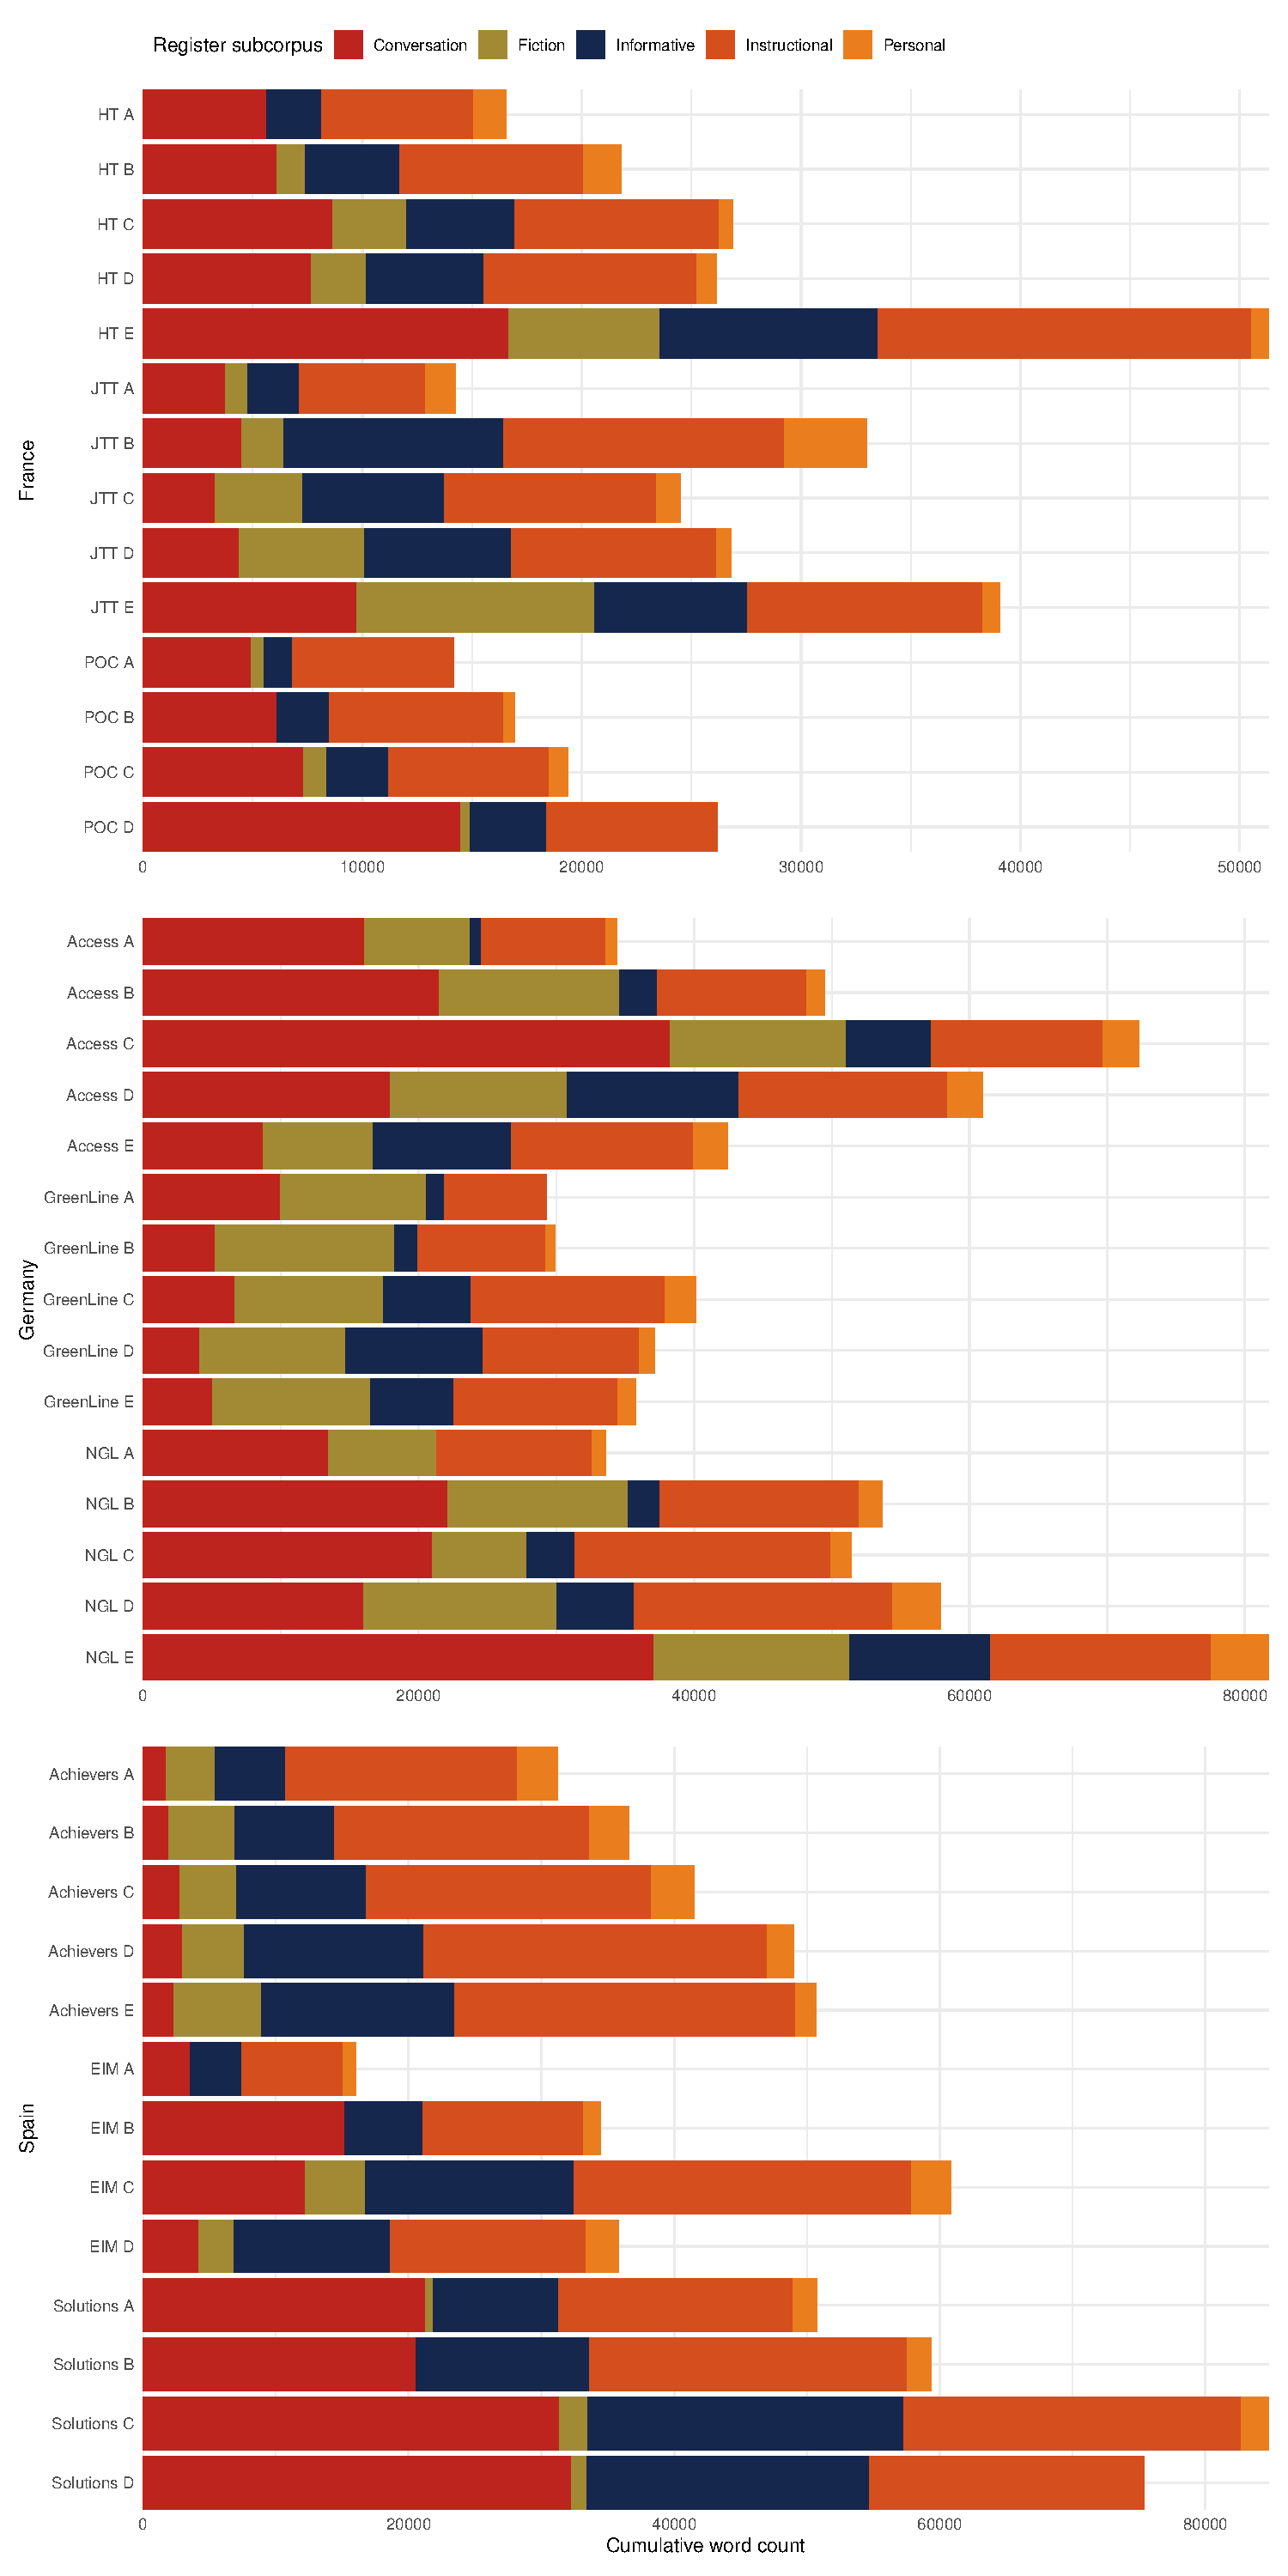
\includegraphics{Ch6_data_prep_files/figure-pdf/TEC-metadata-1.pdf}

\begin{Shaded}
\begin{Highlighting}[]
\CommentTok{\#ggsave(here("plots", "TEC{-}T\_wordcounts\_book.svg"), width = 8, height = 12)}
\end{Highlighting}
\end{Shaded}

The following table provides information about the proportion of
instructional language featured in each textbook series.

\begin{Shaded}
\begin{Highlighting}[]
\NormalTok{metadataInstr }\OtherTok{\textless{}{-}}\NormalTok{ TxBcounts }\SpecialCharTok{|\textgreater{}}  
  \FunctionTok{select}\NormalTok{(Country, Series, Level, Register, Words) }\SpecialCharTok{|\textgreater{}}  
  \FunctionTok{filter}\NormalTok{(Register}\SpecialCharTok{==}\StringTok{"Instructional"}\NormalTok{) }\SpecialCharTok{|\textgreater{}}  
  \FunctionTok{mutate}\NormalTok{(}\AttributeTok{Volume =} \FunctionTok{paste}\NormalTok{(Series, Register)) }\SpecialCharTok{|\textgreater{}}  
  \FunctionTok{mutate}\NormalTok{(}\AttributeTok{Volume =} \FunctionTok{fct\_rev}\NormalTok{(Volume)) }\SpecialCharTok{|\textgreater{}}  
  \FunctionTok{mutate}\NormalTok{(}\AttributeTok{Volume =} \FunctionTok{fct\_reorder}\NormalTok{(Volume, }\FunctionTok{as.numeric}\NormalTok{(Level))) }\SpecialCharTok{|\textgreater{}}  
  \FunctionTok{group\_by}\NormalTok{(Volume, Register) }\SpecialCharTok{|\textgreater{}}  
  \FunctionTok{mutate}\NormalTok{(}\AttributeTok{InstrWordcount =} \FunctionTok{sum}\NormalTok{(Words)) }\SpecialCharTok{|\textgreater{}}  
  \FunctionTok{ungroup}\NormalTok{() }\SpecialCharTok{|\textgreater{}}  
  \FunctionTok{distinct}\NormalTok{(Volume, }\AttributeTok{.keep\_all =} \ConstantTok{TRUE}\NormalTok{) }\SpecialCharTok{|\textgreater{}}  
  \FunctionTok{select}\NormalTok{(Series, InstrWordcount)}

\NormalTok{metaWordcount }\OtherTok{\textless{}{-}}\NormalTok{ TxBcounts }\SpecialCharTok{|\textgreater{}}  
  \FunctionTok{select}\NormalTok{(Country, Series, Level, Register, Words) }\SpecialCharTok{|\textgreater{}}  
  \FunctionTok{group\_by}\NormalTok{(Series) }\SpecialCharTok{|\textgreater{}}  
  \FunctionTok{mutate}\NormalTok{(}\AttributeTok{TECwordcount =} \FunctionTok{sum}\NormalTok{(Words)) }\SpecialCharTok{|\textgreater{}}  
  \FunctionTok{ungroup}\NormalTok{() }\SpecialCharTok{|\textgreater{}}  
  \FunctionTok{distinct}\NormalTok{(Series, }\AttributeTok{.keep\_all =} \ConstantTok{TRUE}\NormalTok{) }\SpecialCharTok{|\textgreater{}}  
  \FunctionTok{select}\NormalTok{(Series, TECwordcount)}

\NormalTok{wordcount }\OtherTok{\textless{}{-}} \FunctionTok{merge}\NormalTok{(metaWordcount, metadataInstr, }\AttributeTok{by =} \StringTok{"Series"}\NormalTok{)}

\NormalTok{wordcount }\SpecialCharTok{|\textgreater{}}  
  \FunctionTok{mutate}\NormalTok{(}\AttributeTok{InstrucPercent =}\NormalTok{ InstrWordcount}\SpecialCharTok{/}\NormalTok{TECwordcount}\SpecialCharTok{*}\DecValTok{100}\NormalTok{) }\SpecialCharTok{|\textgreater{}}  
  \FunctionTok{arrange}\NormalTok{(InstrucPercent) }\SpecialCharTok{|\textgreater{}}  
  \FunctionTok{mutate}\NormalTok{(}\AttributeTok{InstrucPercent =} \FunctionTok{round}\NormalTok{(InstrucPercent, }\DecValTok{2}\NormalTok{)) }\SpecialCharTok{|\textgreater{}}  
  \FunctionTok{kable}\NormalTok{(}\AttributeTok{col.names =} \FunctionTok{c}\NormalTok{(}\StringTok{"Textbook Series"}\NormalTok{, }\StringTok{"Total words"}\NormalTok{, }\StringTok{"Instructional words"}\NormalTok{, }\StringTok{"\% of textbook content"}\NormalTok{), }
        \AttributeTok{digits =} \DecValTok{2}\NormalTok{, }
        \AttributeTok{format.args =} \FunctionTok{list}\NormalTok{(}\AttributeTok{big.mark =} \StringTok{","}\NormalTok{))}
\end{Highlighting}
\end{Shaded}

\begin{longtable}[]{@{}
  >{\raggedright\arraybackslash}p{(\columnwidth - 6\tabcolsep) * \real{0.2286}}
  >{\raggedleft\arraybackslash}p{(\columnwidth - 6\tabcolsep) * \real{0.1714}}
  >{\raggedleft\arraybackslash}p{(\columnwidth - 6\tabcolsep) * \real{0.2857}}
  >{\raggedleft\arraybackslash}p{(\columnwidth - 6\tabcolsep) * \real{0.3143}}@{}}
\toprule\noalign{}
\begin{minipage}[b]{\linewidth}\raggedright
Textbook Series
\end{minipage} & \begin{minipage}[b]{\linewidth}\raggedleft
Total words
\end{minipage} & \begin{minipage}[b]{\linewidth}\raggedleft
Instructional words
\end{minipage} & \begin{minipage}[b]{\linewidth}\raggedleft
\% of textbook content
\end{minipage} \\
\midrule\noalign{}
\endhead
\bottomrule\noalign{}
\endlastfoot
Access & 259,679 & 60,938 & 23.47 \\
NGL & 278,316 & 79,312 & 28.50 \\
GreenLine & 172,267 & 54,263 & 31.50 \\
Solutions & 270,278 & 87,829 & 32.50 \\
JTT & 137,557 & 48,375 & 35.17 \\
HT & 142,676 & 51,550 & 36.13 \\
POC & 76,714 & 30,548 & 39.82 \\
EIM & 147,185 & 59,928 & 40.72 \\
Achievers & 208,978 & 109,886 & 52.58 \\
\end{longtable}

\bookmarksetup{startatroot}

\chapter{Summary}\label{summary}

In summary, this book has no content whatsoever.

\bookmarksetup{startatroot}

\chapter*{References}\label{references}
\addcontentsline{toc}{chapter}{References}

\markboth{References}{References}

\phantomsection\label{refs}
\begin{CSLReferences}{1}{0}
\bibitem[\citeproctext]{ref-associationforcomputingmachinery2020}
Association for Computing Machinery, (ACM). 2020. {``Artifact Review and
Badging Version 1.1.''}
\url{https://www.acm.org/publications/policies/artifact-review-and-badging-current}.

\bibitem[\citeproctext]{ref-berez-kroeker2018}
Berez-Kroeker, Andrea L., Lauren Gawne, Susan Smythe Kung, Barbara F.
Kelly, Tyler Heston, Gary Holton, Peter Pulsifer, et al. 2018.
{``Reproducible Research in Linguistics: A Position Statement on Data
Citation and Attribution in Our Field.''} \emph{Linguistics} 56 (1):
1--18. \url{https://doi.org/10.1515/ling-2017-0032}.

\bibitem[\citeproctext]{ref-diwersy2014}
Diwersy, Sascha, Stephanie Evert, and Stella Neumann. 2014. {``A Weakly
Supervised Multivariate Approach to the Study of Language Variation.''}
In, edited by Benedikt Szmrecsanyi and Bernhard Wälchli, 174--204.
Berlin: De Gruyter.

\bibitem[\citeproctext]{ref-lefoll2021}
Le Foll, Elen. 2021a. \emph{Introducing the Multi-Feature Tagger of
English (MFTE)}. Osnabrück University.
\url{https://github.com/elenlefoll/MultiFeatureTaggerEnglish}.

\bibitem[\citeproctext]{ref-lefoll2021a}
---------. 2021b. \emph{Introducing the Multi-Feature Tagger of English
(MFTE)}. Osnabrück University.
\url{https://github.com/elenlefoll/MultiFeatureTaggerEnglish}.

\bibitem[\citeproctext]{ref-lefoll2024}
---------. 2024. {``Why We Need Open Science and Open Education to
Bridge the Corpus Research{\textendash}practice Gap.''} In, edited by
Peter Crosthwaite, 142--56. London: Routledge.

\bibitem[\citeproctext]{ref-love2019}
Love, Robbie, Vaclav Brezina, Tony McEnery, Abi Hawtin, Andrew Hardie,
and Claire Dembry. 2019. {``Functional Variation in the Spoken BNC2014
and the Potential for Register Analysis.''} \emph{Register Studies} 1
(2): 296--317. \url{https://doi.org/10.1075/rs.18013.lov}.

\bibitem[\citeproctext]{ref-love2017}
Love, Robbie, Claire Dembry, Andrew Hardie, Vaclav Brezina, and Tony
McEnery. 2017. {``The Spoken BNC2014.''} \emph{International Journal of
Corpus Linguistics} 22 (3): 319--44.
https://doi.org/\url{https://doi.org/10.1075/ijcl.22.3.02lov}.

\bibitem[\citeproctext]{ref-mcmanus2021}
McManus, Kevin. 2021. {``Are Replication Studies Infrequent Because of
Negative Attitudes? Insights from a Survey of Attitudes and Practices in
Second Language Research.''} \emph{Studies in Second Language
Acquisition}, December, 1--14.
\url{https://doi.org/10.1017/S0272263121000838}.

\bibitem[\citeproctext]{ref-neumann2021}
Neumann, Stella, and Stephanie Evert. 2021. {``A Register Variation
Perspective on Varieties of English.''} In, edited by Elena Seoane and
Douglas Biber, 144178. Studies in Corpus Linguistics 103. Amsterdam:
Benjamins.

\bibitem[\citeproctext]{ref-rcoreteam2022}
R Core Team. 2022. {``R: A Language and Environment for Statistical
Computing.''} Vienna, Austria. \url{https://www.R-project.org/}.

\bibitem[\citeproctext]{ref-wilkinson2016}
Wilkinson, Mark D., Michel Dumontier, IJsbrand Jan Aalbersberg,
Gabrielle Appleton, Myles Axton, Arie Baak, Niklas Blomberg, et al.
2016. {``The FAIR Guiding Principles for Scientific Data Management and
Stewardship.''} \emph{Scientific Data} 3 (1): 160018.
\url{https://doi.org/10.1038/sdata.2016.18}.

\end{CSLReferences}



\end{document}
